% changelog: "0.5.0, 2024-08-15, Davide Donanzan, Stesura Architettura"

\documentclass[8pt]{article}
\usepackage[italian]{babel}
\usepackage[utf8]{inputenc}
\usepackage[letterpaper, left=1in, right=1in, bottom=0.75in, top=0.75in]{geometry}
\usepackage{amsmath}
\usepackage{subfiles}
\usepackage{lipsum}
\usepackage{csquotes}
\usepackage{amsfonts}
\usepackage[sfdefault]{plex-sans}
\usepackage{float}
\usepackage{pifont}
\usepackage{mathabx}
\usepackage[euler]{textgreek}
\usepackage{makecell}
\usepackage{tikz}
\usepackage{wrapfig}
\usepackage{siunitx}
\usepackage{amssymb} 
\usepackage{tabularx}
\usepackage{adjustbox}
\usepackage[document]{ragged2e}
\usepackage{floatflt}
\usepackage[hidelinks]{hyperref}
\usepackage{graphicx}
\usepackage{hyperref}
\setcounter{tocdepth}{4}
\usepackage{caption}
\usepackage{multicol}
\usepackage{tikz}
\setlength\parindent{0pt}
\captionsetup{font=footnotesize}
\usepackage{fancyhdr} 
\usepackage{graphicx}
\usepackage{capt-of}% 
\usepackage{booktabs}
\usepackage{varwidth}
\usepackage{datetime2}
\usepackage{xcolor}
\usepackage{longtable}
\usepackage{array}
\usepackage{ragged2e}
\usepackage{colortbl}
\usepackage{verbatim}
\usepackage{enumitem}
\setcounter{tocdepth}{4}

\newcommand{\customtitle}{SPECIFICA TECNICA}% o ESTERNO

% -- STILE COLONNA CENTRATA PER TABELLE -- %
\newcolumntype{M}[1]{>{\centering\arraybackslash}m{#1}}

% -- STILE INTESTAZIONE -- %
\fancypagestyle{mystyle}{
	\fancyhf{} 
	\fancyhead[R]{
\includegraphics[height=1cm]{template/images/logos/NaN1fy_logo.png}} 
	\fancyhead[L]{\leftmark} 
	\renewcommand{\headrulewidth}{1pt} 
	\fancyhead[L]{\customtitle} 
	\renewcommand{\headsep}{1.3cm} 
	\fancyfoot[C]{\thepage} 
}

% -- PER LA FIRMA -- %
\newcommand{\signatureline}[1]{%
	 \par\vspace{0.5cm}
	\noindent\makebox[\linewidth][r]{\rule{0.2\textwidth}{0.5pt}\hspace{3cm}\makebox[0pt][r]{\vspace{3pt}\footnotesize #1}}%
}

% -- PER IL GLOSSARIO -- %
\newcommand{\glossterm}[1]{#1\textsuperscript{G}} % inserisci \glossterm{termine}

% -- per abilitare 4x sottosezioni es 2.1.1.1
\setcounter{secnumdepth}{4}
\newcommand{\subsubsubsection}[1]{\paragraph{#1}\mbox{}\\\\}

\begin{document}
\definecolor{myblue}{RGB}{23,103,162}
\begin{titlepage}
	\begin{tikzpicture}[remember picture, overlay]
		\node[anchor=south east, opacity=0.2, yshift = -4cm, xshift= 2em] at (current page.south east) {
\includegraphics[width=0.7\textwidth, trim=0cm 0cm 5cm 0cm, clip]{template/images/logos/Universita_Padova_transparent.png}}; 
		\node[anchor=north west, opacity=1, yshift = 4.2cm, xshift= 1.4cm, scale=1.6] at (current page.south west) {
\includegraphics[width=4cm]{template/images/logos/NaN1fy_logo.png}};
	\end{tikzpicture}
	
	\begin{minipage}[t]{0.47\textwidth}
		{\large{\textsc{Destinatari}}
			\vspace{3mm}
			\\ \large{\textsc{Prof. Tullio Vardanega}}
			\\ \large{\textsc{Prof. Riccardo Cardin}}
		}
	\end{minipage}
	\hfill
	\begin{minipage}[t]{0.47\textwidth}\raggedleft
		{\large{\textsc{Redattori}}
			\vspace{3mm}
			{\\\large{\textsc{Davide Donanzan}\\}} % massimo due 
			{\large{\textsc{Pietro Busato}}}
			
			
		}
		\vspace{8mm}
		
		{\large{\textsc{Verificatori}}
			\vspace{3mm}
			{\\\large{\textsc{Guglielmo Barison}\\}} 
			{\large{\textsc{Veronica Tecchiati}\\}} 
			{\large{\textsc{XXXX XXXX}\\}}
			
		}
		\vspace{2mm}\vspace{2mm}
	\end{minipage}
	\vspace{4cm}
	\begin{center}
		\begin{flushright}
			{\fontsize{30pt}{52pt}\selectfont \textbf{Specifica Tecnica}} % o ESTERNO
		\end{flushright}
		\vspace{3cm}
	\end{center}
	\vspace{10 cm}
	{\small \textsc{\href{mailto: nan1fyteam.unipd@gmail.com}{nan1fyteam.unipd@gmail.com}}}
\end{titlepage}
\pagestyle{mystyle}
\section*{Registro delle Modifiche}
\begin{table}[ht!]	
	\centering
	\begin{tabular}{p{1.2cm} p{2cm} p{5cm} p{3cm} p{3cm}}
		\toprule
		\textbf{Versione}& \textbf{Data} & \textbf{Descrizione} & \textbf{Redattore} & \textbf{Verificatore} \\
		\midrule
  		    0.5.0 & 2024-08-15 & Continuazione sezione \ref{sec:arc}. & Pietro Busato &  \\\\
  		    0.4.0 & 2024-08-12 & Stesura sezione \ref{sec:arc} e \ref{sec:dep}. & Pietro Busato & Veronica Tecchiati \\\\
  		    0.3.0 & 2024-08-10 & Completamento sezione \ref{sec:trac}. & Davide Donanzan & Pietro Busato \\\\
  		    0.2.0 & 2024-08-09 & Continuazione sezione \ref{sec:tec} e stesura sezione \ref{sec:trac}. & Davide Donanzan & Pietro Busato \\\\
		    0.1.0 & 2024-07-25 & Stesura sezione \ref{sec:tec}. & Davide Donanzan & Guglielmo Barison \\\\
    		0.0.0 & 2024-07-01 & Stesura struttura e sezione \ref{sec:intro}. & Davide Donanzan & Guglielmo Barison \\
		\bottomrule
		% Ruolo Redattore o Verificatore
	\end{tabular}
	\caption*{Tabella: Registro delle modifiche.}
	\label{table:Registro delle modifiche}
\end{table}
\newpage
\tableofcontents
\newpage
\listoffigures
\newpage
\listoftables
\newpage
\justifying
\section{Introduzione}\label{sec:intro}
\subsection{Scopo del documento}
Il presente documento si propone come risorsa esaustiva per la comprensione degli aspetti
tecnici chiave del progetto SyncCity. La sua finalità primaria è fornire una descrizione
dettagliata e approfondita dell’\glossterm{architettura} implementativa del \glossterm{sistema}. 
In particolare, si prevede un’analisi approfondita che si estenda anche al livello di design più
basso, includendo definizione e spiegazione dettagliata dei \glossterm{design pattern} utilizzati.\\
L’obiettivo principale del presente documento è triplice:
motivare le scelte di sviluppo adottate; fungere da guida fondamentale per l’attività di codifica e di manutenzione; monitorare la copertura dei requisiti identificati nel
documento \textit{Analisi dei Requisiti}. \\
L’adeguatezza del documento e dell’architettura viene costantemente monitorata e modificata sulla base dei
requisiti e dei feedback ricevuti da parte della \glossterm{Proponente}.
\subsection{Scopo del prodotto}
L'obiettivo del progetto SyncCity è quello di creare una piattaforma atta al monitoraggio
di sensori sparsi geograficamente nel territorio di una città. I sensori in questione
permettono la misurazione e segnalazione di dati \glossterm{real-time} riguardanti le più disparate
caratteristiche e necessità del territorio quali temperatura ed umidità esterna, occupazione di
stalli di parcheggio, funzionamento o guasto elettrico di colonnine di ricarica, traffico stradale e via
dicendo. La Proponente richiede la simulazione di alcuni dei sensori nominati nonchè la
gestione dei dati, della loro persistenza e della loro rappresentazione grafica attraverso \glossterm{widget} e
grafici. 
\\\\SyncCity permetterà un miglioramento della \glossterm{qualità} dei servizi offerti dalla città attraverso il continuo monitoraggio della stessa, ottenendo, gestendo e successivamente condividendo i dati con gli utenti. 
\subsection{Glossario}
Per garantire chiarezza nel linguaggio utilizzato nei documenti, è stato redatto un Glossario contenente le definizioni dei termini con significato specifico da disambiguare. Tali termini sono contrassegnati con una G ad apice. L'inserimento di un termine nel Glossario è considerato completo solo dopo averne fornito la definizione.
\subsection{Riferimenti}
\subsubsection{Normativi}
\begin{itemize}
	\item \textit{Norme di Progetto v2.0.0};
	\item Presentazione e documentazione del \glossterm{capitolato} d’appalto C6 - SyncCity:
	\begin{itemize}
		\item \href{https://www.math.unipd.it/~tullio/IS-1/2023/Progetto/C6p.pdf}{\color{myblue}https://www.math.unipd.it\textasciitilde{}tullio/IS-1/2023/Progetto/C6p.pdf} (Ultimo accesso: \today)
		\item \href{https://www.math.unipd.it/~tullio/IS-1/2023/Progetto/C6.pdf}{\color{myblue}https://www.math.unipd.it/\textasciitilde{}tullio/IS-1/2023/Progetto/C6.pdf} (Ultimo accesso: \today)
	\end{itemize}
	\item Regolamento di progetto:
	\begin{itemize}
		\item \href{https://www.math.unipd.it/~tullio/IS-1/2023/Dispense/PD2.pdf}{\color{myblue}https://www.math.unipd.it/\textasciitilde{}tullio/IS-1/2023/Dispense/PD2.pdf} (Ultimo accesso: \today)
	\end{itemize}
\end{itemize}
\clearpage
\subsubsection{Informativi}
\begin{itemize}
    \item \textit{Analisi dei Requisiti v2.0.0};
    \item \textit{Glossario v2.0.0};
    \item Diagrammi delle classi (UML) - corso di Ingegneria del Software a.a. 2023/2024:
    \begin{itemize}
        \item \href{https://www.math.unipd.it/~rcardin/swea/2023/Diagrammi%20delle%20Classi.pdf}{\color{myblue}https://www.math.unipd.it/\textasciitilde{}rcardin/swea/2023/Diagrammi\%20delle\%20Classi.pdf} (Ultimo accesso: \today)
    \end{itemize}
    \item Diagrammi di Sequenza (UML) - corso di Ingegneria del Software a.a. 2023/2024:
    \begin{itemize}
        \item \href{https://www.math.unipd.it/~rcardin/swea/2022/Diagrammi%20di%20Sequenza.pdf}{\color{myblue}https://www.math.unipd.it/\textasciitilde{}rcardin/swea/2022/Diagrammi\%20di\%20Sequenza.pdf} (Ultimo accesso: \today)
    \end{itemize}
    \item Progettazione - corso di Ingegneria del Software a.a. 2023/2024:
    \begin{itemize}
        \item \href{https://www.math.unipd.it/~tullio/IS-1/2023/Dispense/T6.pdf}{\color{myblue}https://www.math.unipd.it/\textasciitilde{}tullio/IS-1/2023/Dispense/T6.pdf} (Ultimo accesso: \today)
    \end{itemize}
\end{itemize}
\subsubsection{Tecnici}
\begin{itemize}
    \item Documentazione \glossterm{Docker}:
    \begin{itemize}
		\item \href{https://docs.docker.com/}{\color{myblue}https://docs.docker.com/} (Ultimo accesso: \today)
	\end{itemize}
    \item Documentazione \glossterm{Docker Compose}:
    \begin{itemize}
		\item \href{https://docs.docker.com/compose/}{\color{myblue}https://docs.docker.com/compose/} (Ultimo accesso: \today)
	\end{itemize}
    \item Documentazione \glossterm{Python}:
    \begin{itemize}
		\item \href{https://docs.python.org/3/}{\color{myblue}https://docs.python.org/3/} (Ultimo accesso: \today)
	\end{itemize}
    \item Documentazione pytest - \glossterm{Python}:
    \begin{itemize}
		\item \href{https://docs.pytest.org/en/7.1.x/contents.html}{\color{myblue}https://docs.pytest.org/en/7.1.x/contents.html} (Ultimo accesso: \today)
	\end{itemize}
    \item Documentazione unittest - \glossterm{Python}:
    \begin{itemize}
		\item \href{https://docs.python.org/3/library/unittest.html}{\color{myblue}https://docs.python.org/3/library/unittest.html} (Ultimo accesso: \today)
	\end{itemize}
    \item Documentazione numpy - \glossterm{Python}:
    \begin{itemize}
		\item \href{https://numpy.org/devdocs/user/}{\color{myblue}https://numpy.org/devdocs/user/} (Ultimo accesso: \today)
	\end{itemize}
    \item Documentazione confluent-kafka - \glossterm{Python}:
    \begin{itemize}
		\item \href{https://developer.confluent.io/get-started/python/}{\color{myblue}https://developer.confluent.io/get-started/python/} (Ultimo accesso: \today)
	\end{itemize}
    \item Documentazione clickhouse-connect - \glossterm{Python}:
    \begin{itemize}
		\item \href{https://clickhouse.com/docs/en/integrations/python}{\color{myblue}https://clickhouse.com/docs/en/integrations/python} (Ultimo accesso: \today)
	\end{itemize}
    \item Documentazione Apache \glossterm{Kafka}:
    \begin{itemize}
		\item \href{https://kafka.apache.org/20/documentation.html}{\color{myblue}https://kafka.apache.org/20/documentation.html} (Ultimo accesso: \today)
	\end{itemize}
    \item Documentazione Apache \glossterm{Flink}:
    \begin{itemize}
		\item \href{https://nightlies.apache.org/flink/flink-docs-stable/}{\color{myblue}https://nightlies.apache.org/flink/flink-docs-stable/} (Ultimo accesso: \today)
	\end{itemize}
    \item Documentazione \glossterm{Java}:
    \begin{itemize}
		\item \href{https://docs.oracle.com/en/java/}{\color{myblue}https://docs.oracle.com/en/java/} (Ultimo accesso: \today)
	\end{itemize}
    \item Documentazione Apache \glossterm{Maven}:
    \begin{itemize}
		\item \href{https://maven.apache.org/guides/index.html}{\color{myblue}https://maven.apache.org/guides/index.html} (Ultimo accesso: \today)
	\end{itemize}
    \item Documentazione \glossterm{ClickHouse}:
    \begin{itemize}
		\item \href{https://clickhouse.com/docs/en/intro}{\color{myblue}https://clickhouse.com/docs/en/intro} (Ultimo accesso: \today)
	\end{itemize}
    \item Documentazione Kafka Engine - \glossterm{ClickHouse}:
    \begin{itemize}
		\item \href{https://clickhouse.com/docs/en/engines/table-engines/integrations/kafka}{\color{myblue}https://clickhouse.com/docs/en/engines/table-engines/integrations/kafka} (Ultimo accesso: \today)
	\end{itemize}
    \item Documentazione materialized view - \glossterm{ClickHouse}:
    \begin{itemize}
		\item \href{https://clickhouse.com/docs/en/guides/developer/cascading-materialized-views}{\color{myblue}https://clickhouse.com/docs/en/guides/developer/cascading-materialized-views} (Ultimo accesso: \today)
	\end{itemize}
    \item Documentazione MergeTree - \glossterm{ClickHouse}:
    \begin{itemize}
		\item \href{https://clickhouse.com/docs/en/engines/table-engines/mergetree-family/mergetree#mergetree}{\color{myblue}https://clickhouse.com/docs/en/engines/table-engines/mergetree-family/mergetree\#mergetree} (Ultimo accesso: \today)
	\end{itemize}
    \item Documentazione \glossterm{Grafana}:
    \begin{itemize}
		\item \href{https://grafana.com/docs/grafana/latest}{\color{myblue}https://grafana.com/docs/grafana/latest} (Ultimo accesso: \today)
	\end{itemize}
    \item Documentazione ClickHouse datasource - \glossterm{Grafana}:
    \begin{itemize}
		\item \href{https://grafana.com/grafana/plugins/grafana-clickhouse-datasource/}{\color{myblue}https://grafana.com/grafana/plugins/grafana-clickhouse-datasource/} (Ultimo accesso: \today)
	\end{itemize}
    \item Documentazione variables - \glossterm{Grafana}:
    \begin{itemize}
		\item \href{https://grafana.com/docs/grafana/latest/variables/}{\color{myblue}https://grafana.com/docs/grafana/latest/variables/} (Ultimo accesso: \today)
	\end{itemize}
    \item Documentazione alerts - \glossterm{Grafana}:
    \begin{itemize}
		\item \href{https://grafana.com/docs/grafana/latest/alerting/}{\color{myblue}https://grafana.com/docs/grafana/latest/alerting/} (Ultimo accesso: \today)
	\end{itemize}
    \item Documentazione notification policies - \glossterm{Grafana}:
    \begin{itemize}
		\item \href{https://grafana.com/docs/grafana/latest/alerting-rules/create-notification-policy/}{\color{myblue}https://grafana.com/docs/grafana/latest/alerting-rules/create-notification-policy/} (Ultimo accesso: \today)
	\end{itemize}
\end{itemize}
\newpage
\clearpage
\section{Tecnologie}\label{sec:tec}
In questa sezione verranno illustrati gli strumenti e le tecnologie impiegati per lo sviluppo del software nonché infrastrutture, linguaggi di programmazione, \glossterm{librerie} e \glossterm{framework} utilizzati.
\subsection{\glossterm{Docker}}
In fase di sviluppo, testing e produzione, sono stati utilizzati \glossterm{container} \glossterm{Docker} per creare ambienti di lavoro efficaci e consistenti.
\subsubsection{Ambienti}
Sono stati creati quattro ambienti di lavoro con focus operativi differenti.
\begin{itemize}
    \item \textbf{Ambiente di produzione:}
    \begin{itemize}
        \item Ambiente dove i programmatori possono testare il codice nella produzione dei dati simulati;
        \item Il focus è quello della produzione dei dati simulati nell'ottica della fruizione del servizio fornito dall'applicativo.
        \item L'intera \glossterm{data pipeline} ad esclusione dello \glossterm{stream-processing}, è in funzione.
    \end{itemize}
    \item \textbf{Ambiente di development:}
    \begin{itemize}
        \item Ambiente dove i programmatori possono controllare il corretto collegamento tra le tecnologie implementate;
        \item Non è attiva la generazione dei dati simulati;
        \item Il focus è l'interazione fra le tecnologie della \glossterm{data pipeline}.
    \end{itemize}
    \item \textbf{Ambiente di test:}
    \begin{itemize}
        \item Ambiente che simula l'ambiente di produzione;
        \item Utilizza test automatizzati per verificare la correttezza del codice nelle sue unità e nell'integrazione di queste tra loro.
    \end{itemize}
     \item \textbf{Ambiente di stream-processing:}
    \begin{itemize}
        \item Ambiente dove i programmatori possono controllare il corretto funzionamento dello \glossterm{stream-processing};
        \item Il focus è quello di osservare il comportamento, implementare e verificare l'elaborazione di stream differenti;
        \item L'intera \glossterm{data pipeline} ad esclusione della visualizzazione dei dati, è in funzione.
    \end{itemize}
\end{itemize}
\subsubsection{Images}
Di seguito sono elencate le immagini \glossterm{Docker} utilizzate:
\begin{itemize}
    \item \textbf{\glossterm{Python}}
    \begin{itemize}
        \item \textbf{Image:} python:3.11-bookworm
        \item \textbf{Riferimento:}  \href{https://hub.docker.com/layers/library/python/3.11-bookworm/images/sha256-94c2dca43c9c127e42dfd021039cc83d8399752097612b49bdc7b00716b6d826}{\color{myblue}https://hub.docker.com/layers/library/python/3.11-bookworm/images/sha256-94c2dca43c9c127e42dfd021039cc83d8399752097612b49bdc7b00716b6d826} (Ultimo accesso: \today)
        \item \textbf{Ambiente:}
        \begin{itemize}
            \item Produzione;
            \item Test;
            \item Stream processing.
        \end{itemize}
    \end{itemize}
    \clearpage
    \item \textbf{Apcahe \glossterm{Kafka}}
    \begin{itemize}
        \item \textbf{Image:} bitnami/kafka:3.7.0
        \item \textbf{Riferimento:}  \href{https://hub.docker.com/r/bitnami/kafka}{\color{myblue}https://hub.docker.com/r/bitnami/kafka} (Ultimo accesso: \today)
        \item \textbf{Ambiente:}
        \begin{itemize}
            \item Produzione;
            \item Test;
            \item Stream processing.
        \end{itemize}
    \end{itemize}
    \item \textbf{Apache \glossterm{Flink}}
    \begin{itemize}
        \item \textbf{Image:} flink:1.18.1-java17 
        \item \textbf{Riferimento:} \href{https://hub.docker.com/_/flink}{\color{myblue}https://hub.docker.com/\_/flink} (Ultimo accesso: \today)
        \item \textbf{Ambiente:}
        \begin{itemize}
            \item Produzione;
            \item Development;
            \item Stream processing.
        \end{itemize}
    \end{itemize}
    \item \textbf{\glossterm{ClickHouse}}
    \begin{itemize}
        \item \textbf{Image:} clickhouse/clickhouse-server:latest
        \item \textbf{Riferimento:} \href{https://hub.docker.com/r/clickhouse/clickhouse-server}{\color{myblue}https://hub.docker.com/r/clickhouse/clickhouse-server} (Ultimo accesso: \today)
        \item \textbf{Ambiente:}
        \begin{itemize}
            \item Produzione;
            \item Development;
            \item Test;
            \item Stream processing.
        \end{itemize}
    \end{itemize}
    \item \textbf{\glossterm{Grafana}}
    \begin{itemize}
        \item \textbf{Image:} grafana/grafana-oss:latest
        \item \textbf{Riferimento:} \href{https://hub.docker.com/r/grafana/grafana-oss}{\color{myblue}https://hub.docker.com/r/grafana/grafana-oss} (Ultimo accesso: \today)
        \item \textbf{Ambiente:}
        \begin{itemize}
            \item Produzione;
            \item Development.
        \end{itemize}
    \end{itemize}
\end{itemize}
\subsection{Linguaggi e formato dati}
\subsubsection{\glossterm{Python}}
Linguaggio di programmazione ad alto livello, interpretato e multi-paradigma.
\begin{itemize}
    \item \textbf{Versione:} 3.11
    \item \textbf{Documentazione:} \href{https://docs.python.org/3/}{\color{myblue}https://docs.python.org/3/} (Ultimo accesso: \today)
    \item \textbf{Utilizzo:} 
    \begin{itemize}
        \item Simulazione di dati prodotti da sensori di diverso tipo;
        \item Test di unità per singole classi o funzioni;
        \item Test d'integrazione tra generatore dati, broker e database utilizzati;
        \item Calcolo dei valori per metriche di qualità di prodotto.
    \end{itemize}
    \clearpage
    \item \textbf{Librerie e framework:}   
    \begin{itemize}
        \item \textbf{pytest}
        \begin{itemize}
            \item \textbf{Versione:} 8.0.2
            \item \textbf{Documentazione:} \href{https://docs.pytest.org/en/7.1.x/contents.html}{\color{myblue}https://docs.pytest.org/en/7.1.x/contents.html} (Ultimo accesso: \today)
            \item \textbf{Utilizzo:} Scrittura di codice per test d'integrazione agevolata grazie a funzioni di before\_test e after\_test e la gestione di fixture.
        \end{itemize}
        \item \textbf{unittest}
        \begin{itemize}
            \item \textbf{Versione:} 3.11
            \item \textbf{Documentazione:} \href{https://docs.python.org/3/library/unittest.html}{\color{myblue}https://docs.python.org/3/library/unittest.html} (Ultimo accesso: \today)
            \item \textbf{Utilizzo:} Scrittura di script di test d'unità agevolati dall'uso di patch, asserzioni e set up di casistiche di testing.
        \end{itemize}
        \item \textbf{numpy}
        \begin{itemize}
            \item \textbf{Versione:} 1.26.4
            \item \textbf{Documentazione:} \href{https://numpy.org/devdocs/user/}{\color{myblue}https://numpy.org/devdocs/user/} (Ultimo accesso: \today)
            \item \textbf{Utilizzo:} Fornitura di strutture dati e operazioni matematiche e statistiche complesse.
        \end{itemize}
        \item \textbf{confluent-kafka}
        \begin{itemize}
            \item \textbf{Versione:} 2.3.0
            \item \textbf{Documentazione:} \href{https://developer.confluent.io/get-started/python/}{\color{myblue}https://developer.confluent.io/get-started/python/} (Ultimo accesso: \today)
            \item \textbf{Utilizzo:} Fornitura di strumenti per la produzione e consumo di messaggi da parte di Apache Kafka
        \end{itemize}
        \item \textbf{clickhouse-connect}
        \begin{itemize}
            \item \textbf{Versione:} 0.7.2
            \item \textbf{Documentazione:} \href{https://clickhouse.com/docs/en/integrations/python}{\color{myblue}https://clickhouse.com/docs/en/integrations/python} (Ultimo accesso: \today)
            \item \textbf{Utilizzo:} Fornitura di strumenti che semplificano l'interazione con il database ClickHouse permettendo query e inserimenti nel database.
        \end{itemize}
    \end{itemize}
\end{itemize}
\subsubsection{\glossterm{SQL}}
Linguaggio standard per la gestione e la manipolazione dei database.
\begin{itemize}
    \item \textbf{Utilizzo:}
    \begin{itemize}
        \item Creazione delle tabelle del database in base al topic, ovvero la tipologia di sensore;
        \item Gestione e interrogazione del database \glossterm{ClickHouse}.
    \end{itemize}
\end{itemize}
\subsubsection{\glossterm{JSON}}
Formato per lo scambio di dati, basato sui concetti di oggetto (insieme di coppie chiave-valore) e di array (lista di oggetti, stringhe, valori o array).
\begin{itemize}
    \item \textbf{Utilizzo:}
    \begin{itemize}
        \item Formato dei messaggi trasmessi dal simulatore dei sensori a \glossterm{Kafka};
        \item Configurazione delle dashboard e dei pannelli in \glossterm{Grafana}.
    \end{itemize}
\end{itemize}
\subsubsection{\glossterm{Java}}
Linguaggio di programmazione ad alto livello, orientato agli oggetti e a tipizzazione statica
\begin{itemize}
    \item \textbf{Versione:} 17
    \item \textbf{Documentazione:} \href{https://docs.oracle.com/en/java/}{\color{myblue}https://docs.oracle.com/en/java/} (Ultimo accesso: \today)
    \item \textbf{Utilizzo:}
    \begin{itemize}
        \item Implementazione di \glossterm{Flink};
        \item Gestione ed elaborazione di dati provenienti da topic di \glossterm{Kafka};
        \item Reindirizzamento di dati elaborati verso un topic di Kafka.
    \end{itemize}
\end{itemize}
\subsubsection{\glossterm{YAML}}
Formato di serializzazione leggibile dall’uomo utilizzato per rappresentare dati strutturati in modo chiaro e semplice.
\begin{itemize}
    \item \textbf{Utilizzo:}
    \begin{itemize}
        \item Configurazione file \glossterm{Docker Compose};
        \item Configurazione \glossterm{Github} workflow e actions; 
        \item Configurazione provisioning \glossterm{Grafana} e politiche di alerting;
        \item Configurazione di \glossterm{Flink}.
    \end{itemize}
\end{itemize}
    \subsubsection{\glossterm{XML}}
 Metalinguaggio per la definizione di linguaggi di markup, ovvero un linguaggio basato su un meccanismo sintattico che consente di definire e controllare il significato degli elementi contenuti in un documento o in un testo.
\begin{itemize}
    \item \textbf{Utilizzo:}
    \begin{itemize}
        \item Definizione di timezone nella configurazione di \glossterm{ClickHouse};
        \item Definizione di dettagli di configurazione nel POM (Porject Object Model) per l'elaborazione degli stream in Java.
    \end{itemize}
\end{itemize}
\subsection{Servizi della pipeline}
\subsubsection{Apache \glossterm{Kafka}}
Apache Kafka è una piattaformaG open-source di streaming distribuito sviluppata
dall’Apache Software Foundation. Progettata per gestire flussi di dati in tempo reale in modo scalabile e affidabile, è ampiamente utilizzata nel data streaming e nell’integrazione dei dati nelle moderne applicazioni.
\begin{itemize}
    \item \textbf{Versione:} 3.7.0
    \item \textbf{Documentazione:} \href{https://kafka.apache.org/20/documentation.html}{\color{myblue}https://kafka.apache.org/20/documentation.html} (Ultimo accesso: \today)
    \item \textbf{Utilizzo} 
    \\Nel nostro prodotto Kafka agisce da broker, ricevendo i dati dai produttori, ovvero il generatore di dati in \glossterm{python} e rendendoli disponibili ai consumer. I consumer sono due:
    \begin{itemize}
        \item \glossterm{ClickHouse:} i dati vengono resi disponibili per essere archiviati nel database suddivisi per topic;
        \item \glossterm{Flink:} i dati sono resi disponibili per analisi e elaborazione in tempo reale attraverso \glossterm{stream processing}.
    \end{itemize}
    I dati provenienti dalle simulazioni dei sensori vengono inviati a Kafka come messaggi in formato JSON.
\end{itemize}
\subsubsection{Apache \glossterm{Flink}}
Apache Flink è un framework per l'elaborazione di flussi e l'elaborazione in batch open-source sviluppato da Apache Software Foundation. Il nucleo di Flink è un motore di flusso di dati in streaming distribuito scritto in Java e Scala.
\begin{itemize}
    \item \textbf{Versione:} 1.18.1
    \item \textbf{Documentazione:} \href{https://nightlies.apache.org/flink/flink-docs-stable/}{\color{myblue}https://nightlies.apache.org/flink/flink-docs-stable/} (Ultimo accesso: \today)
    \item \textbf{Utilizzo}
    \\Nel prodotto, Flink agisce da consumer degli stream dati simulati dal generatore \glossterm{python} e ottenuti da \glossterm{Kafka}, detto producer. Ottenuti gli stream li elabora e inserisce in un nuovo e apposito topic di Kafka.
    \end{itemize}
\subsubsection{\glossterm{ClickHouse}}
Clickhouse è un \glossterm{sistema} di gestione di database (DBMS) di tipo colonnare,
progettato per l’analisi di grandi volumi di dati grazie a query SQL in tempo reale.
\begin{itemize}
    \item \textbf{Versione:} 24.2.1.2248
    \item \textbf{Documentazione:} \href{https://clickhouse.com/docs/en/intro}{\color{myblue}https://clickhouse.com/docs/en/intro} (Ultimo accesso: \today)
    \item \textbf{Utilizzo}
    \\Nel progetto, Clickhouse ha in carico la persistenza dei dati provenienti dai sensori recuperarndo in tempo reale i dati da \glossterm{Kafka}, assicurandone l'immediata disponibilità per l’analisi.
    Clickhouse è in grado di organizzare e grandi volumi di dati in modo rapido e incrementale, grazie all'architettura colonnare.
    Grafana, infine, raccoglie tali dati per la rappresentazione grafica, tramite query SQL.
\end{itemize}
\subsubsection{\glossterm{Grafana}}
Grafana è una piattaforma open-source per la visualizzazione e l'analisi interattiva di dati, utilizzata per creare \glossterm{dashboard} e grafici da fonti di dati eterogenee
\begin{itemize}
    \item \textbf{Versione:} 10.4.0
    \item \textbf{Documentazione:} \href{https://grafana.com/docs/grafana/latest}{\color{myblue}https://grafana.com/docs/grafana/latest} (Ultimo accesso: \today)
    \item \textbf{Utilizzo}
    \\Nel progetto Grafana viene utilizzato per la visualizzazione dei dati tramite \glossterm{dashboard} e grafici interattivi consentendo il monitoraggio in tempo reale dei sensori.
    Permette inoltre l'analisi di tali dati, fornendo strumenti statistici e opzioni di filtraggio. Infine, offre la possibilità di introdurre un sistema di alerting basato sul verificarsi condizioni anomale per un tempo prolungato, inviando una notifica sulla piattaforma \glossterm{Discord}.
\end{itemize}
\newpage
\section{Architettura di sistema}\label{sec:arc}
\subsection{Modello architetturale}
L'applicativo basa il funzionamento sulla gestione e sull'elaborazione di stream continui di dati eterogenei in tempo reale ma fornendo, al tempo stesso, la possibilità di immagazzinare tali dati per un'analisi su più larga scala di batch dati. Per sviluppare tale \glossterm{sistema} abbiamo adottato la \glossterm{k-architecture}.
\subsubsection{\glossterm{k-architecture}}
L’architettura Kappa è un modello di elaborazione e processamento per la gestione di stream di dati che offre un’alternativa all’architettura Lambda. La caratteristica principale di questa architettura è permettere lo sviluppo sia di stream processing che di batch processing all’interno di un unico stack tecnologico, mantenendo il \glossterm{sistema} in real time.
\subsubsection{Vantaggi}
\begin{itemize}
    \item Minore complessità nell'implementazione e nella manutenzione;
    \item Maggiore coerenza tra analisi batch e real-time.
\end{itemize}
\subsubsection{Svantaggi}
\begin{itemize}
    \item Rallentamento dovuto all'elaborazione degli stream in tempo-reale;
    \item Meno flessibile dell'architettura Lambda per via di un'unico stack tecnologico sulla quale avviene l'elaborazione dei dati.
\end{itemize}
\subsubsection{Componenti di sistema}
\begin{itemize}
    \item \textbf{Data source:} I dati sono generati dal simulatore dei sensori dislocati geograficamente sul territorio della città. La generazione dei dati è \glossterm{event driven}, quindi basata sul verificarsi di eventi, i quali possono anche corrispondere ad un intervallo di tempo regolare. Il dato generato viene passato sottoforma di messaggio allo streaming layer; 
    \item \textbf{Streaming layer:} Lo streaming layer è composto da Apache \glossterm{Kafka}, un \glossterm{sistema} di messaggistica distribuito che riceve i dati dai sensori e li gestisce trattandoli come stream. Successivamente li rende disponibili per l’elaborazione in tempo reale nello streaming layer e per l'archiviazione nello storage layer; 
    \item \textbf{Processing layer:} Il processing layer è costituito da Apache \glossterm{Flink} che consuma i dati dallo streaming layer e li processa in tempo reale. Successivamente ritorna lo stream allo streaming layer per archiviarlo;
    \item \textbf{Storage layer:} Lo storage layer è costituito dal database colonnare \glossterm{ClickHouse}, che archivia i dati in arrivo dallo streaming layer e li rende disponibili per l’analisi e la visualizzazione sia in tempo reale che batch nel data visualization layer;
    \item \textbf{Data visualization layer:} Il data visualization layer è composto da \glossterm{Grafana}, piattaforma di visualizzazione dei dati che si occupa della rappresentazine degli stessi ottenuti dallo storage layer e della gestione delle notifiche in caso di anomalie.
\end{itemize}
\clearpage
\subsection{Data-flow}
Il diagramma presentato qui di seguito rappresenta il percorso compiuto da una qualsiasi unità di dati all'interno del sistema, a quali operazioni esso è sottoposto, come viene elaborato e dove viene infine archiviato e utilizzato. Il diagramma mostra dunque anche le connessioni tra le varie parti del sistema e come esse interagiscono tra di loro.
\begin{itemize}
    \item \textbf{Generazione dati:} I dati, prodotti nella realtà dal rilevamento di sensori fisici, vengono qui simulati attraverso dei generatori verosimili nel loro funzionamento e campionamento. I dati generati vengono trasportati poi al broker \glossterm{Kafka} in formato \glossterm{JSON} e indirizzati ai rispettivi topic.
    \item \textbf{Stream processing e instradamento:} Una volta arrivati su \glossterm{Kafka} e indirizzati sui topic di appartenenza, i dati vengono direttamente instradati e archiviati su \glossterm{ClickHouse} tramite Kafka Engine, materialized view e MergeTree. \\
    Alcuni dati possono, tuttavia, venire elaborati tramite stream processing attraverso Apache \glossterm{Flink}, prima di venire reimmessi in un topic apposito e quindi archiviati sul database Clickhouse. Nel nostro caso i dati interessati sono: 
    \begin{itemize}
    	\item Temperatura e umidità, sia inviati individualmente che combinati per creare un nuovo tipo di dato, ovvero la temperatura percepita;
    	\item Pagamenti e Soste di un parcheggio, sia inviati individualmente che combinati per creare un nuovo tipo di dato, ovvero l'efficienza parcheggio.
    \end{itemize}
    \item \textbf{Visualizzazione:} I dati, archiviati su \glossterm{ClickHouse}, vengono visualizzati da \glossterm{Grafana} tramite query sulle tabelle, generando \glossterm{dashboard} di visualizzazione per i risultati di tali query.
\end{itemize}
\subsection{Architettura del generatore dati}
Il generatore di dati in \glossterm{pyhton} è una componente che punta a simulare l'acquisizione di dati da parte di sensori fisici dislocati nel suolo cittadino. Non è parte effettiva dello stack tecnologico alla quale il \glossterm{capitolato} punta ma è parte necessaria per il corretto sviluppo dell'applicativo e per l'analisi del funzionamento delle tecnologie implementate. A seguito, verrà presentata l’architettura individuata mediante l’utilizzo di diagrammi delle classi e relative descrizioni e verranno motivate le scelte dei design pattern individuati in quanto scelte progettuali.
\clearpage
\subsubsection{Struttura generale}
La struttura generale del simulatore prevede la presenza di tre moduli. Il modulo dei sensori genera i dati su richiesta del modulo dei thread che a sua volta invoca il modulo writer per inviare il dato generato a \glossterm{Kafka}.
\begin{figure}[h!]
    \centering
    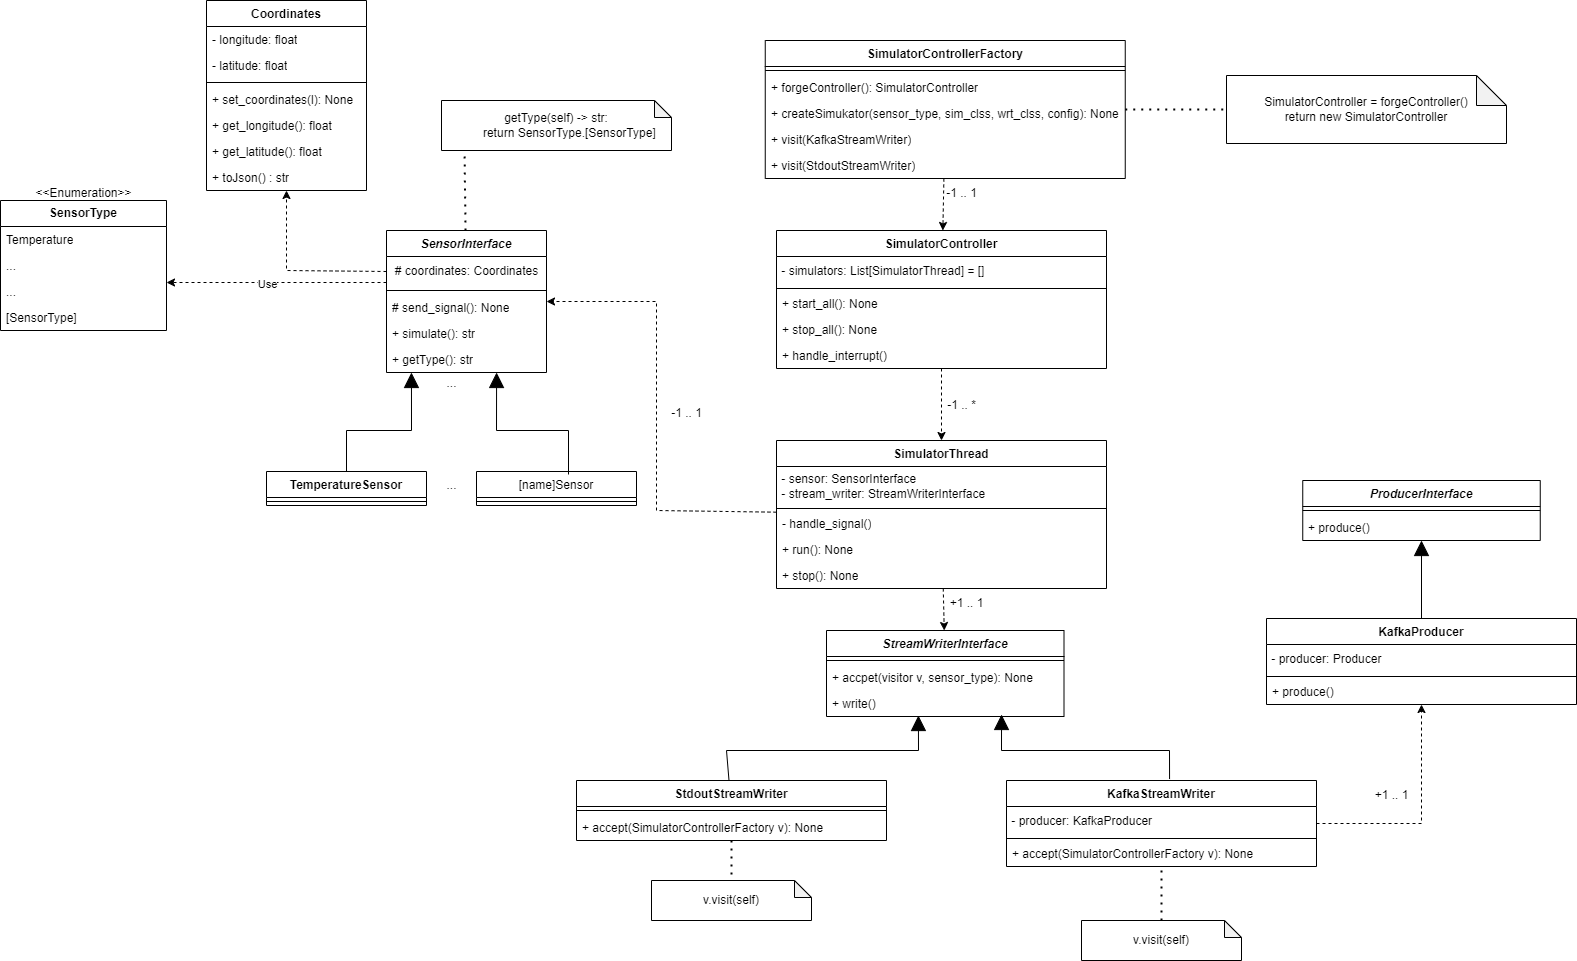
\includegraphics[width=0.8\textwidth]{images_st/overview.png}
    \caption{Diagramma delle classi dell'architettura.}
    \label{fig:Diagramma delle classi dell'architettura}
\end{figure}
Nella figura è presente solo la classe concreta \verb|TemperatureSensor| che implementa \verb|SensorInterface|, poiché le altre sono analoghe.
\subsubsection{Modulo sensori}
\begin{figure}[h!]
    \centering
    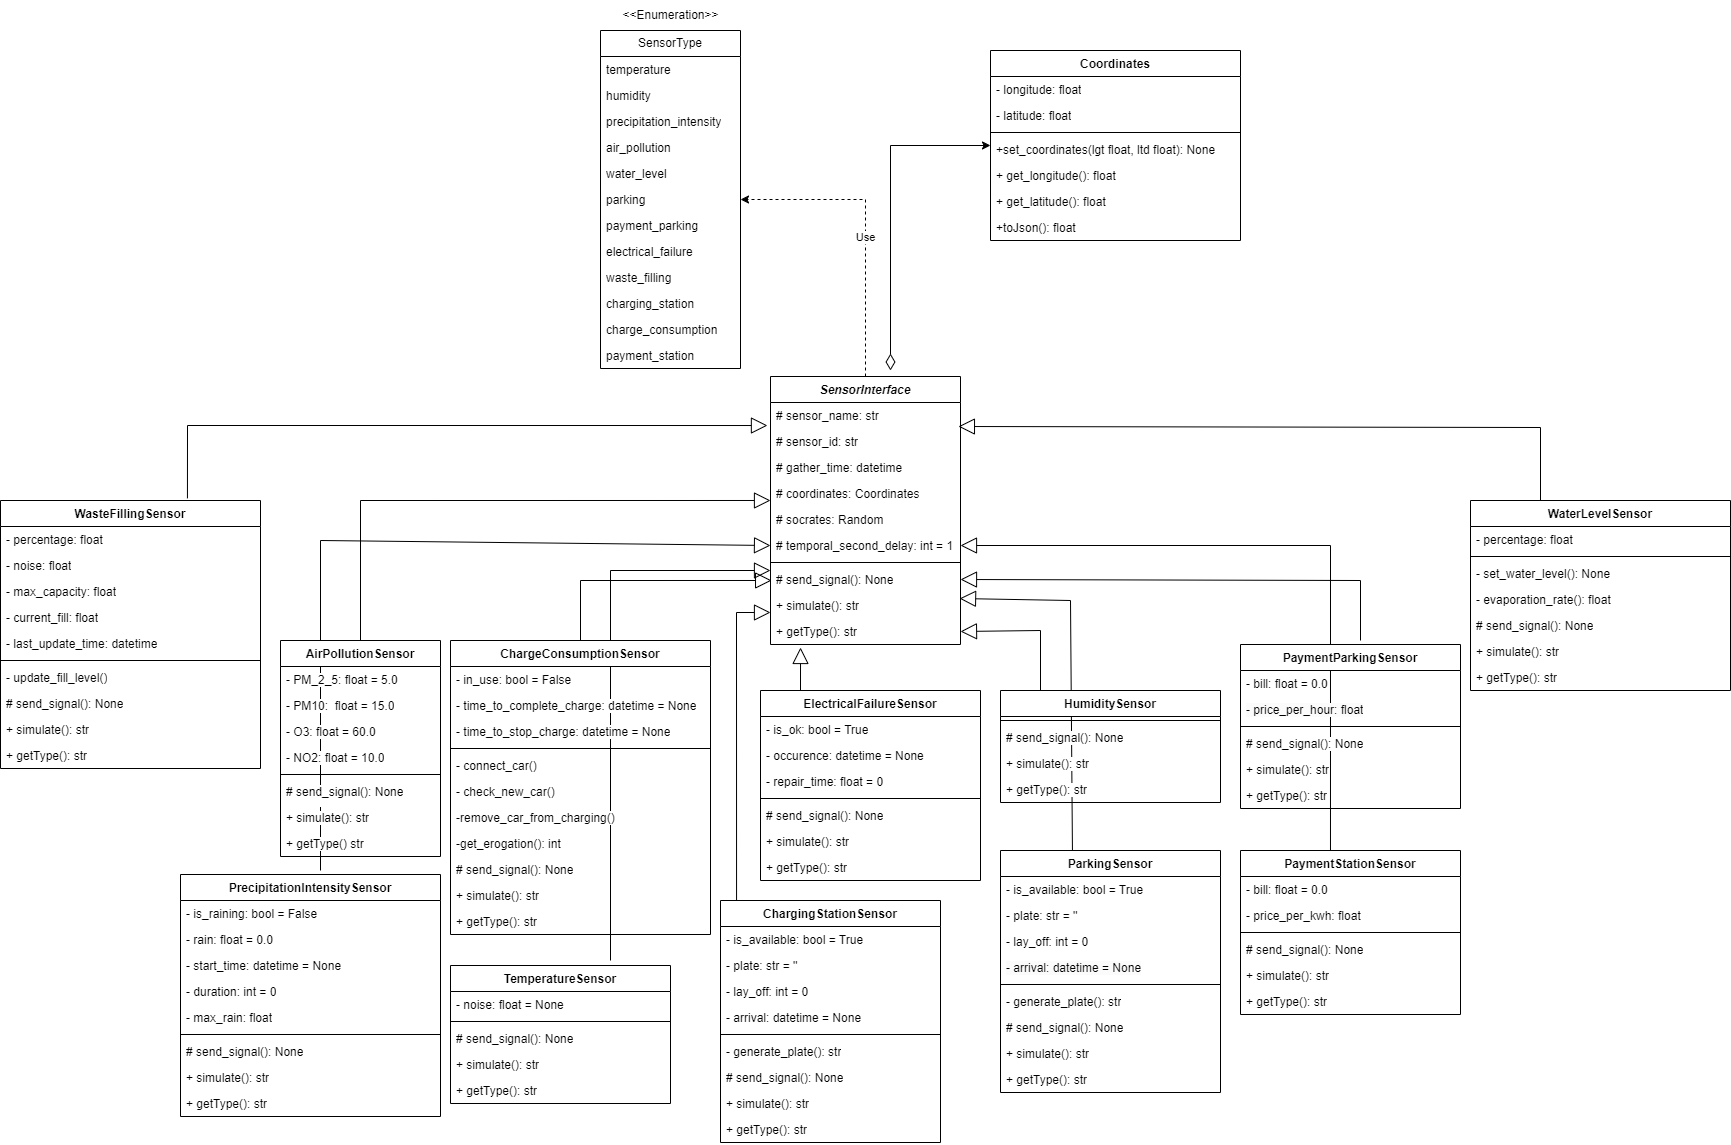
\includegraphics[width=0.8\textwidth]{images_st/sensors.png}
    \caption{Diagramma delle classi del modulo sensori.}
    \label{fig:Diagramma delle classi del modulo sensori}
\end{figure}
Questo modulo si occupa della generazione dei dati da parte di simulatori verosimili. Lo scopo è quindi quello di diversificare la generazione del dato rispetto ad un interfaccia comune tra tutti i sensori.
Design pattern utilizzati: 
\begin{itemize}
    \item \textbf{Template method:} 
    \\Questo pattern è implementato nella classe astratta \verb|SensorInterface| la quale offre il comportamento generico di tutti i sensori. Le classi che estendono \verb|SensorInterface| implementano i metodi astratti defininendo un comportamento specifico al tipo di sensore.
    Questo permette una facile estensione del codice nel caso venga aggiunta una tipologia di sensore e previene la duplicazione di codice. I metodi principali implementati nelle sottoclassi sono due:
    \begin{itemize}
        \item \textbf{simulate():} Genera il dato secondo una logica specifica al tipo di sensore e lo restituisce sottoforma di stringa \glossterm{JSON} come valore di ritorno al thread per la sua scrittura;
        \item \textbf{send\_signal():} Metodo protetto che decide la politica di occorrenza di un evento per uno specifico tipo di sensore. Esso può essere un intervallo periodico di tempo, il verificarsi di una condizione casuale o una combinazione dei due. Questo metodo segnala al thread la necessità di effettuare la scrittura di un nuovo dato. 
    \end{itemize}
\end{itemize}
Le classi implementate sono:
\begin{itemize}
    \item \textbf{SensorInterface}
    \begin{itemize}
        \item \textbf{Attributi:}
        \begin{itemize}
            \item \textbf{sensor\_name: string[protected]} - Nome del sensore;
            \item \textbf{sensor\_id: string[protected]} - ID del sensore;
            \item \textbf{gather\_time: datetime[protected]} - Oggetto per metodi datetime;
            \item \textbf{coorinates: Coorinates[protected]} - Coordinate del sensore;
            \item \textbf{socrates: Random[protected]} - Oggetto per metodi randomici;
            \item \textbf{temporal\_second\_delay: int[protected]} - Delay tra le misurazioni.
        \end{itemize}
        \item \textbf{Metodi:}
        \begin{itemize}
            \item \textbf{getId(): string[public]} - Funzione che ritorna l'ID del sensore;
            \item \textbf{simulate(): string[public]} - Metodo astratto per la generazione del dato;
            \item \textbf{send\_signal(): void[protected]} - Metodo per la definizione del meccanismo di evento;
            \item \textbf{getType(): string[public]} - Funzione che ritorna il tipo di sensore.
        \end{itemize}
    \end{itemize}
    \item \textbf{TemperatureSensor}
    \begin{itemize}
        \item \textbf{Attributi:}
        \begin{itemize}
            \item \textbf{noise: float[private]} - Rumore nei dati.
        \end{itemize}
        \item \textbf{Metodi:}
        \begin{itemize}
            \item \textbf{simulate(): string[public]} - Metodo che genera il valore di temeperatura in gradi Celsius;
            \item \textbf{send\_signal(): None[protected]} - Metodo per che definisce l'intervallo di tempo tra due simulazioni consecutive;
            \item \textbf{getType(): string[public]} - Funzione che ritorna il tipo di sensore.
        \end{itemize}
    \end{itemize}
    \item \textbf{HumiditySensor}
    \begin{itemize}
        \item \textbf{Metodi:}
        \begin{itemize}
            \item \textbf{simulate(): string[public]} - Metodo che genera il valore di umidità relativa in percentuale;
            \item \textbf{send\_signal(): None[protected]} - Metodo per che definisce l'intervallo di tempo tra due simulazioni consecutive;
            \item \textbf{getType(): string[public]} - Funzione che ritorna il tipo di sensore.
        \end{itemize}
    \end{itemize}
    \item \textbf{PrecipitationIntensitySensor}
    \begin{itemize}
        \item \textbf{Attributi:}
        \begin{itemize}
            \item \textbf{is\_raining: bool[private]} - Presenza o meno di pioggia;
            \item \textbf{rain: float[private]} - Valore attuale di intensità;
            \item \textbf{start\_time: datetime[private]} - Momento di inizio della pioggia;
            \item \textbf{duration: int[private]} - Secondi di durata della pioggia;
            \item \textbf{max\_rain: float[private]} - Massima intensità.
        \end{itemize}
        \item \textbf{Metodi:}
        \begin{itemize}
            \item \textbf{simulate(): string[public]} - Metodo che genera il valore di intensità in mm/h;
            \item \textbf{send\_signal(): None[protected]} - Metodo per che definisce l'intervallo di tempo tra due simulazioni consecutive;
            \item \textbf{getType(): string[public]} - Funzione che ritorna il tipo di sensore.
        \end{itemize}
    \end{itemize}
    \item \textbf{AirPollutionSensor}
    \begin{itemize}
        \item \textbf{Attributi:}
        \begin{itemize}
            \item \textbf{PM\_2\_5: float[private]} - Valore di particolato 2.5;
            \item \textbf{PM\_10: float[private]} - Valore di particolato 10;
            \item \textbf{O3: float[private]} - Valore di ozono;
            \item \textbf{NO2: float[private]} - Valore di diossido di azoto.
        \end{itemize}
        \item \textbf{Metodi:}
        \begin{itemize}
            \item \textbf{simulate(): string[public]} - Metodo che genera il valore di inquinamento dell'aria in µg / $\mbox{m}^{\mbox{3}}$;
            \item \textbf{send\_signal(): None[protected]} - Metodo per che definisce l'intervallo di tempo tra due simulazioni consecutive;
            \item \textbf{getType(): string[public]} - Funzione che ritorna il tipo di sensore.
        \end{itemize}
    \end{itemize}
    \item \textbf{WaterLevelSensor}
    \begin{itemize}
        \item \textbf{Attributi:}
        \begin{itemize}
            \item \textbf{percentage: float[private]} - Valore del livello dell'acqua.
        \end{itemize}
        \item \textbf{Metodi:}
        \begin{itemize}
            \item \textbf{simulate(): string[public]} - Metodo che genera il valore del livello dell'acqua in percentuale;
            \item \textbf{send\_signal(): None[protected]} - Metodo per che definisce l'intervallo di tempo tra due simulazioni consecutive;
            \item \textbf{getType(): string[public]} - Funzione che ritorna il tipo di sensore.
        \end{itemize}
    \end{itemize}
    \item \textbf{ParkingSensor}
    \begin{itemize}
        \item \textbf{Attributi:}
        \begin{itemize}
            \item \textbf{is\_available: bool[private]} - Disponibilità del parcheggio;
            \item \textbf{plate: string[private]} - Targa dell'occupante;
            \item \textbf{lay\_off: int[private]} - Tempo di occupazione;
            \item \textbf{arrival: datetime[private]} - Momento di arrivo.
        \end{itemize}
        \item \textbf{Metodi:}
        \begin{itemize}
            \item \textbf{generate\_plate(): string[private]} - Metodo che genera una targa di un possibile occupante;
            \item \textbf{simulate(): string[public]} - Metodo che genera la possibilità di occupazione di uno stallo, la targa di chi lo occupa, il periodo di occupazione e il momento in cui è stato occupato;
            \item \textbf{send\_signal(): None[protected]} - Metodo per che definisce l'evento di segnalazione come l'occupazione o la liberazione di uno stallo;
            \item \textbf{getType(): string[public]} - Funzione che ritorna il tipo di sensore.
        \end{itemize}
    \end{itemize}
    \item \textbf{PaymentParkingSensor}
    \begin{itemize}
        \item \textbf{Attributi:}
        \begin{itemize}
            \item \textbf{bill: float[private]} - Pagamento dovuto;
            \item \textbf{price\_per\_hour: float[private]} - Prezzo all'ora.
        \end{itemize}
        \item \textbf{Metodi:}
        \begin{itemize}
            \item \textbf{simulate(): string[public]} - Metodo che genera il valore del pagamento dovuto in euro;
            \item \textbf{send\_signal(): None[protected]} - Metodo per che definisce l'intervallo di tempo tra segnalazioni consecutive;
            \item \textbf{getType(): string[public]} - Funzione che ritorna il tipo di sensore.
        \end{itemize}
    \end{itemize}
    \item \textbf{ElectricalFailureSensor}
    \begin{itemize}
        \item \textbf{Attributi:}
        \begin{itemize}
            \item \textbf{is\_ok: bool[private]} - Presenza o meno di un gausto;
            \item \textbf{repair\_time: float[private]} - Tempo necessario a riparare un guasto;
            \item \textbf{occurence: datetime[private]} - Momento di occorenza di un guasto.
        \end{itemize}
        \item \textbf{Metodi:}
        \begin{itemize}
            \item \textbf{simulate(): string[public]} - Metodo che genera l'occorenza di un guasto, il tempo necessario a ripararlo e il momento in cui è occorso;
            \item \textbf{send\_signal(): None[protected]} - Metodo per che definisce l'evento di segnalazione come l'occorrere e la riparazione di un guasto;
            \item \textbf{getType(): string[public]} - Funzione che ritorna il tipo di sensore.
        \end{itemize}
    \end{itemize}
    \item \textbf{WasteFillingSensor}
    \begin{itemize}
        \item \textbf{Attributi:}
        \begin{itemize}
            \item \textbf{percentage: float[private]} - Valore di riempimento dell'isola ecologica;
            \item \textbf{noise: float[private]} - Rumore nei dati;
            \item \textbf{max\_capacity: float[private]} - Capacità massima;
            \item \textbf{current\_fill: float[private]} - Riempimento attuale;
            \item \textbf{last\_update\_time: datetime[private]} - Ultimo aggiornamento.
        \end{itemize}
        \item \textbf{Metodi:}
        \begin{itemize}
            \item \textbf{update\_fill\_level(): void[private]} - Metodo che aggiorna il valore di riempimento in base all'orario;
            \item \textbf{simulate(): string[public]} - Metodo che genera il valore di rimepimento dell'isola ecologica in percentuale;
            \item \textbf{send\_signal(): None[protected]} - Metodo per che definisce l'intervallo di tempo tra due segnalazioni consecutive;
            \item \textbf{getType(): string[public]} - Funzione che ritorna il tipo di sensore.
        \end{itemize}
    \end{itemize}
    \item \textbf{ChargingStationSensor}
    \begin{itemize}
        \item \textbf{Attributi:}
        \begin{itemize}
            \item \textbf{is\_available: bool[private]} - Disponibilità della colonnina;
            \item \textbf{plate: string[private]} - Targa dell'occupante;
            \item \textbf{lay\_off: int[private]} - Tempo di occupazione;
            \item \textbf{arrival: datetime[private]} - Momento di arrivo.
        \end{itemize}
        \item \textbf{Metodi:}
        \begin{itemize}
            \item \textbf{generate\_plate(): string[private]} - Metodo che genera una targa di un possibile occupante;
            \item \textbf{simulate(): string[public]} - Metodo che genera la possibilità di occupazione di una colonnina, la targa di chi la occupa, il periodo di occupazione e il momento in cui è stata occupata;
            \item \textbf{send\_signal(): None[protected]} - Metodo per che definisce l'evento di segnalazione come l'occupazione o la liberazione di una colonnina;
            \item \textbf{getType(): string[public]} - Funzione che ritorna il tipo di sensore.
        \end{itemize}
    \end{itemize}
    \item \textbf{PaymentStationSensor}
    \begin{itemize}
        \item \textbf{Attributi:}
        \begin{itemize}
            \item \textbf{bill: float[private]} - Pagamento dovuto;
            \item \textbf{price\_per\_hour: float[private]} - Prezzo all'ora.
        \end{itemize}
        \item \textbf{Metodi:}
        \begin{itemize}
            \item \textbf{simulate(): string[public]} - Metodo che genera il valore del pagamento dovuto in euro;
            \item \textbf{send\_signal(): None[protected]} - Metodo per che definisce l'intervallo di tempo tra segnalazioni consecutive;
            \item \textbf{getType(): string[public]} - Funzione che ritorna il tipo di sensore.
        \end{itemize}
    \end{itemize}
    \item \textbf{ChargeConsumptionSensor}
    \begin{itemize}
        \item \textbf{Attributi:}
        \begin{itemize}
            \item \textbf{in\_use: bool[private]} - Utilizzo o meno della colonnina;
            \item \textbf{time\_to\_complete\_charge: datetime[private]} - Tempo alla quale si completa la carica;
            \item \textbf{time\_to\_stop\_charge: datetime[private]} - Tempo alla quale si ferma la carica;
            \item \textbf{next\_connection: datatime[private]} - Tempo alla quale si collega la prossima macchina;
            \item \textbf{mean\_erogation\_power: float[private]} - Erogazione media.
        \end{itemize}
        \item \textbf{Metodi:}
        \begin{itemize}
            \item \textbf{connect\_car(): void[private]} - Metodo che collega la macchina alla colonnina;
            \item \textbf{remove\_car\_from\_charging(): void[private]} - Metodo che scollega la macchina dalla colonnina;
            \item \textbf{check\_new\_car(): void[private]} - Metodo che controlla la disponibilità della colonnina;
            \item \textbf{get\_erogation(): int[private]} - Metodo che ritorna l'erogazione della colonnina;
            \item \textbf{simulate(): string[public]} - Metodo che genera il valore di consumo di una colonnina di ricarica in kWh;
            \item \textbf{send\_signal(): None[protected]} - Metodo per che definisce l'intervallo di tempo tra due segnalazioni consecutive;
            \item \textbf{getType(): string[public]} - Funzione che ritorna il tipo di sensore.
        \end{itemize}
    \end{itemize}
\end{itemize}
\subsubsection{Modulo writer}
\begin{figure}[h!]
    \centering
    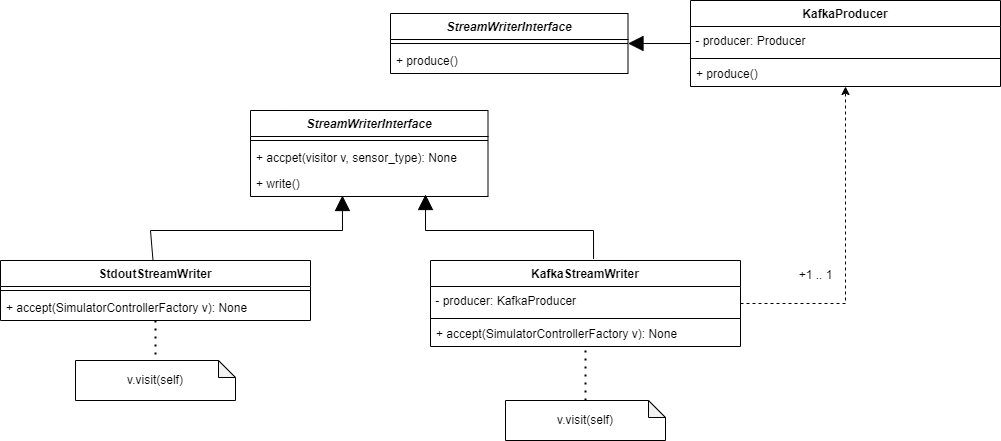
\includegraphics[width=0.8\textwidth]{images_st/writer.png}
    \caption{Diagramma delle classi del modulo writer.}
    \label{fig:Diagramma delle classi del modulo writer}
\end{figure}
Questo modulo ha il compito di effettuare la scrittura di informazioni su diversi tipi di servizi indipendentemente dal meccanismo di simulazione dei sensori.
Design pattern utilizzati: 
\begin{itemize}
    \item \textbf{Strategy:} 
    \\Questo pattern è implementato nella classe astratta \verb|StreamWriterInterface| la quale offre diverse strategie per la scrittura dei dati. Sono state implementate due sottoclassi concrete:
    \begin{itemize}
        \item \textbf{StdoutStreamWriter:} Stampa il dato sul terminale;
        \item \textbf{KafkaStreamWriter:} Invia messaggi ai topic di \glossterm{Kafka}. 
    \end{itemize}
    Quest'ultima classe permette la scrittura chiamando un producer. Con ottica di una possibile estensibilità è previsto che il producer chiamato sia un oggetto della classe \verb|KafkaProducer|, estensione della classe \verb|ProducerInterface|.
\end{itemize}
Le classi implementate sono:
\begin{itemize}
    \item \textbf{StreamWriterInterface}
    \begin{itemize}
        \item \textbf{Metodi:}
        \begin{itemize}
            \item \textbf{accept(visitor, sensor\_type): void[public]} - Metodo astratto per accettazione del visitor;
            \item \textbf{write(data: string): void[public]} - Metodo astratto per la scrittura dei dati.
        \end{itemize}
    \end{itemize}
    \item \textbf{StdoutStreamWriter}
    \begin{itemize}
        \item \textbf{Metodi:}
        \begin{itemize}
            \item \textbf{accept(visitor, sensor, sim\_clss, config: Dict): void[public]} - Metodo per accettazione del visitor per standard output;
            \item \textbf{write(data: string): void[public]} - Metodo per la scrittura dei dati su terminale.
        \end{itemize}
    \end{itemize}
    \item \textbf{KafkaStreamWriter}
    \begin{itemize}
        \item \textbf{Attributi:}
        \begin{itemize}
            \item \textbf{producer: KafkaProducer[private]} - Producer Kafka;
            \item \textbf{topic: string[private]} - Topic per Kafka.
        \end{itemize}
        \item \textbf{Metodi:}
        \begin{itemize}
            \item \textbf{accept(visitor, sensor, sim\_clss, config: Dict): void[public]} - Metodo per accettazione del visitor per Kafka ourtput;
            \item \textbf{write(data: string): void[public]} - Metodo per l'invio di dati a topic di Kafka.
        \end{itemize}
    \end{itemize}
    \item \textbf{ProducerInterface}
    \begin{itemize}
        \item \textbf{Metodi:}
        \begin{itemize}
            \item \textbf{produce(data: string, callback: Callable): void[public]} - Metodo astratto per produrre messaggi per Kafka.
        \end{itemize}
    \end{itemize}
    \item \textbf{ProducerInterface}
    \begin{itemize}
        \item \textbf{Attributi:}
        \begin{itemize}
            \item \textbf{producer: Producer[private]} - Producer della libreria confluent-kafka;
            \item \textbf{topic: string[private]} - Topic per Kafka.
        \end{itemize}
        \item \textbf{Metodi:}
        \begin{itemize}
            \item \textbf{produce(data: string, callback: Callable): void[public]} - Metodo per produrre messaggi per Kafka.
        \end{itemize}
    \end{itemize}
\end{itemize}
\subsubsection{Modulo Thread}
\begin{figure}[h!]
    \centering
    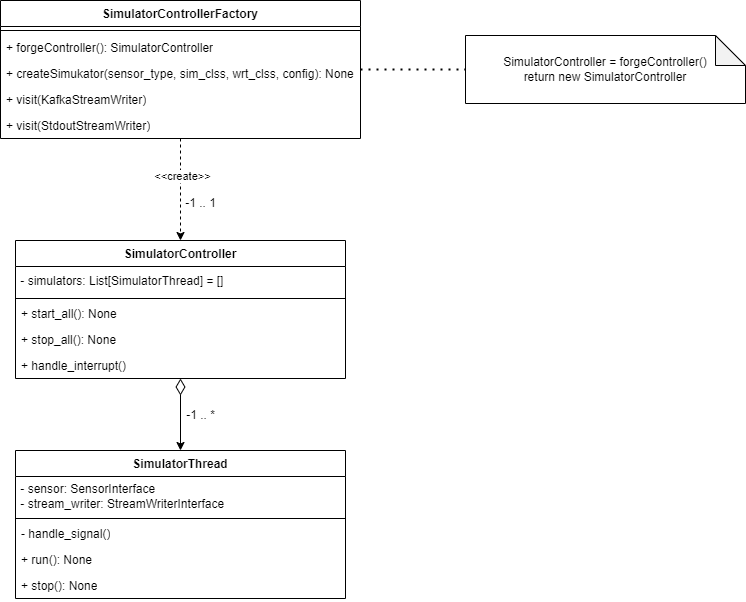
\includegraphics[width=0.8\textwidth]{images_st/threads.png}
    \caption{Diagramma delle classi del modulo thread.}
    \label{fig:Diagramma delle classi del modulo thread}
\end{figure}
Il modulo thread ha lo scopo la gestione dei simulatori come thread asincroni, creati da una factory e gestiti da un controller. Questi funzionano come wrapper dei sensori stessi e hanno il compito di chaimare i writer per la scrittura dei dati generati dai sensori.
Design pattern utilizzati: 
\begin{itemize}
    \item \textbf{Factory Method:} 
    \\Questo pattern è implementato nella classe \verb|SimulatorControllerFactory| la quale ha il compito di creare tanti thread quanti sensori specificati nel file config.json, senza conoscere il tipo del sensore contenuto. Ha il dovere inoltre di creare il controller per la gestione dei thread;
    \item \textbf{Visitor:}
    \\Questo pattern è implementato nella classe \verb|SimulatorControllerFactory| la quale permette di riconoscere la classe concreta dello streamwriter per lo specifico thread da creare. Questa pratica può sembrare poco ortodossa ma facilita l'utilizzo del writer per ogni specifico thread.
\end{itemize}
Le classi implementate sono:
\begin{itemize}
    \item \textbf{SimulatorControllerFactory}
    \begin{itemize}
        \item \textbf{Attributi:}
        \begin{itemize}
            \item \textbf{simulators: List[SimulatorThread][private]} - Lista di thread creati;
            \item \textbf{config\_file: string[private]} - File di configurazione contenente i sensori;
            \item \textbf{stream\_writer: Type[StreamWriterInterface][private]} - Oggetto streamwriter;
            \item \textbf{simulators\_inventory: Dict[str, int][private]} - Inventario dei sensori creati;
            \item \textbf{writers\_kafka\_inventory: Dict[str, KafkaStreamWriter][private]} - Inventario dei tipi di sensori che scrivono su Kafka.
        \end{itemize}
        \item \textbf{Metodi:}
        \begin{itemize}
            \item \textbf{createSimulator(sensor\_type: SensorType, sim\_clss: Type[SensorInterface], wrt\_clss: Type[StreamWriterInterface], config: Dict): int[protected]} - Metodo che crea un thread;
            \item \textbf{visit(writer: StdoutStreamWriter, sensor, sim\_clss, config: Dict): void[public]} - Metodo per la visita di un sensore con uno standard output writer;
            \item \textbf{visit(writer: KafkaStreamWriter, sensor, sim\_clss, config: Dict, sensor\_type: string): void[public]} - Metodo per la visita di un sensore con un kafka writer;
            \item \textbf{forgeContorller(): SimulatorController[public]} - Metodo per la creazione del controller e dei thread da esso gestiti.
        \end{itemize}
    \end{itemize}
    \item \textbf{SimulatorController}
    \begin{itemize}
        \item \textbf{Attributi:}
        \begin{itemize}
            \item \textbf{simulators: List[SimulatorThread][private]} - Lista di thread.
        \end{itemize}
        \item \textbf{Metodi:}
        \begin{itemize}
            \item \textbf{start\_all(): void[public]} - Metodo che fa partire tutti i thread;
            \item \textbf{stop\_all(): void[public]} - Metodo che ferma tutti i thread;
            \item \textbf{handle\_interrupt(): void[public]} - Metodo che gestisce le interruzioni e ferma tutti i thread.
        \end{itemize}
    \end{itemize}
    \item \textbf{SimulatorThread}
    \begin{itemize}
        \item \textbf{Attributi:}
        \begin{itemize}
            \item \textbf{stop\_event: Event[private]} - Evento di interruzione;
            \item \textbf{stream\_writer: StreamWriterInterface[private]} - Streamwriter del thread;
            \item \textbf{sensor: SensorInterface[private]} - Sensore contenuto nel thread.
        \end{itemize}
        \item \textbf{Metodi:}
        \begin{itemize}
            \item \textbf{handle\_signal(): void[private]} - Metodo che scrive il dato generato dal sensore;
            \item \textbf{run(): void[public]} - Metodo che aspetta il segnale per la simulazione del sensore;
            \item \textbf{stop(): void[public]} - Metodo che ferma il thead.
        \end{itemize}
    \end{itemize}
\end{itemize}
\subsubsection{Toolkit}
Il toolkit è un'insieme di funzioni, classi e costanti che abbaimo utilizzato per agevolare determinate operazioni e/o non strettamente collegati ai moduli precedentemente elencati.
Di questo toolkit evidenzieremo:
\begin{itemize}
    \item \textbf{sensor\_type:} Enumerazione contenente tutti i tipi di sensori;
    \item \textbf{Coordinates:} Classe che identifica un oggetto coordinata:
    \begin{itemize}
        \item \textbf{Attributi:}
        \begin{itemize}
            \item \textbf{longitude: float[private]} - Longitudine;
            \item \textbf{latitude: float[private]} - Latitudine;
        \end{itemize}
        \item \textbf{Metodi:}
        \begin{itemize}
            \item \textbf{setCoordinates(longitude: float, latitude: float): None[public]} - Imposta il valore degli attributi;
            \item \textbf{get\_longitude(): float[public]} - Funzione che ritorna la longitudine;
            \item \textbf{get\_latitude(): float[public]} - Funzione che ritorna la latitudine;
            \item \textbf{toJson(): string[public]} - Restituisce il contenuto dell'oggetto sottoforma di stringa \glossterm{JSON}.
        \end{itemize}
    \end{itemize}
    \item \textbf{jsonfy():} Funzione che permette la conversione dei dati di una simulazione in una stringa \glossterm{JSON}.
\end{itemize}
\clearpage
\subsection{\glossterm{Kafka}}
\subsubsection{Topic}
I topic in \glossterm{Kafka} permettono di separare logicamente i diversi tipi di messaggi o eventi prodotti. Per separare le diverse misurazioni dei sensori è stato creato un topic dedicato per ogni tipologia di sensore.
Ciò facilita la creazione all’interno del database \glossterm{ClickHouse} delle tabelle, le quali acquisiscono automaticamente i dati consumandoli da Kafka.
\subsubsection{Formato messaggi}
I messaggi trasmessi a \glossterm{Kafka} sono in formato \glossterm{JSON} e possiedono la seguente struttura:
\begin{verbatim}
    {
        "sensor_type": "Tipo sensore",
        "sensor_name": "Nome sensore",
        "sensor_id": "ID sensore",
        "gather_time": "AAAA-MM-DD HH:MM:SS.ssssss",
        "readings": [Oggetti che contengono i valori della misurazione],
        "coordinates": {"type": "point", "coordinates": [Latitudine, Longitudine]}
    }
\end{verbatim}
\subsubsection{Misurazione sensori}
Gli oggetti contenenti le misurazioni dei sensori presentano forme diverse in base alla quantità di informazioni passate. Nello specifico, alcuni sensori riferiscono un'unica informazione che viene quindi passata con il seguente formato:
\begin{verbatim}
    {
        "type": "Unità di misura", 
        "value": Valore misurato
    }
\end{verbatim}
I sensori che forniscono più informazioni diverse presentano un messaggio nel formato:
\begin{verbatim}
    {
        "prima informazione": Valore
        "seconda informazione": Valore
    }
\end{verbatim}
\subsection{\glossterm{Flink}}
\subsection{\glossterm{ClickHouse}}
Il database ClickHouse ha come scopo quello di memorizzare i dati provenienti dai sensori in modo da poterli analizzare e visualizzare in seguito. I dati vengono acquisiti suddivisi per topic, uno per ogni tipo di sensore, e poi memorizzati nelle apposite tabelle.
\subsubsection{Struttura}
\begin{itemize}
    \item \textbf{Tabella per Kafka topic:} Per ogni tipo di sensore viene creata una tabella contenente una stringa di dati grezzi in formato \glossterm{JSON} per ogni messaggio proveniente dal topic dedicato. Questo tipo di tabelle vengono popolate tramite il ClickHouse Kafka Engine, che inserisce all’interno della tabella i messaggi con il topic corrispondente.
    \\La creazione di tale tabella avviene per provisioning tramite il seguente codice \glossterm{SQL} sostituendo il corretto tipo di sensore:
    \begin{verbatim}
    CREATE TABLE sc_database.topic_sensor_type
    (
        rawJSON String
    ) ENGINE = Kafka('kafka:9092', 'sensor_type', 'SyncCity', 'JSONAsString');
    \end{verbatim}
    \item \textbf{Materialized View:} La materialized view, attraverso funzioni di estrazione, estrapola i valori dai dati grezzi delle topic tables e li assegna alle corrispondenti chiavi. Questa view sarà poi fondamentale per la creazione della tabella effettiva del database contenente i dati archiviati. La materialized view è un meccanismo che agevola le query permettendo un accesso semplificato ai dati. 
    \\Vengono create tramite il seguente codice \glossterm{SQL}, sostituendo il corretto tipo di sensore:
    \begin{verbatim}
        CREATE MATERIALIZED VIEW sc_database.sensor_type_mv
        TO sc_database.sensor_type
        AS
        SELECT
            JSONExtractString(rawJSON, 'sensor_name') AS sensor_name,
            JSONExtractString(rawJSON, 'sensor_id') AS sensor_id,
            toDateTime64(JSONExtractString(rawJSON, 'gather_time'), 0) AS gather_time,
            JSONExtractFloat(rawJSON, 'coordinates', 'coordinates', 1) AS latitude,
            JSONExtractFloat(rawJSON, 'coordinates', 'coordinates', 2) AS longitude,
            JSONExtractTipo_di_value(rawJSON, 'readings', 1, 'value') AS value
        FROM sc_database.topic_sensor_type;
    \end{verbatim}
    \item \textbf{Tabella per sensor\_type:} Attraverso il motore di archiviazione MergeTree, i dati estrapolati nella materialized view vengono archiviati in una apposita tabella che consiste nel vero e proprio storage di dati, suddiviso per tipo di sensori.
    \\La creazione delle tabelle avviene attraverso il seguente codice \glossterm{SQL} sostituendo il corretto tipo di sensore:
    \begin{verbatim}
        CREATE TABLE sc_database.sensor_type
        (
            sensor_name String,
            sensor_id String,
            gather_time DATETIME64,
            latitude Float64,
            longitude Float64,
            value Tipo_di_value
        
        ) ENGINE = MergeTree()
            ORDER BY (sensor_id, gather_time);
    \end{verbatim}
\end{itemize}
\begin{figure}[h!]
    \centering
    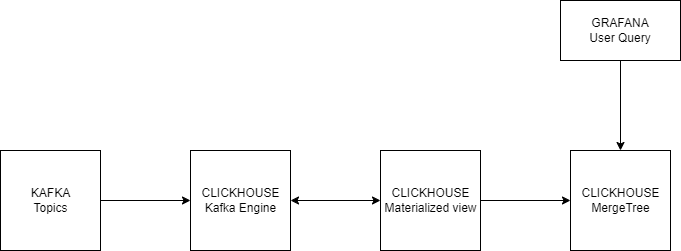
\includegraphics[width=0.8\textwidth]{images_st/kafka-clickhouse.png}
    \caption{Schema collegamento Kafka ClickHouse.}
    \label{fig:Schema collegamento Kafka ClickHouse}
\end{figure}
\subsubsection{Motori di archiviazione}
Nell'ottica dell'archiviazione dei dati provenienti da \glossterm{Kafka}, \glossterm{ClickHouse} offre vari engine. In particolare, due sono stati utilizzati per la creazione delle tabelle per la persistenza dei dati generati:
\begin{itemize}
    \item \textbf{Kafka Engine:} permette di leggere la stringa \glossterm{JSON} contenente i dati grezzi provenienti dal broker e di iniettarla all’interno delle topic tables;
    \item \textbf{MergeTree:} permette di effettuare operazioni di inserimento ed eliminazione in modo efficiente e di effettuare query su intervalli di tempo specifici. Inoltre permette il popolamento delle tabelle con i dati estrapolati nelle materialized view. 
\end{itemize}
\subsubsection{Sensore di temperatura}
Nella tabella per i sensori di temperatura viene salvato in ``readings" il valore di temperatura generato.
\begin{figure}[h!]
    \centering
    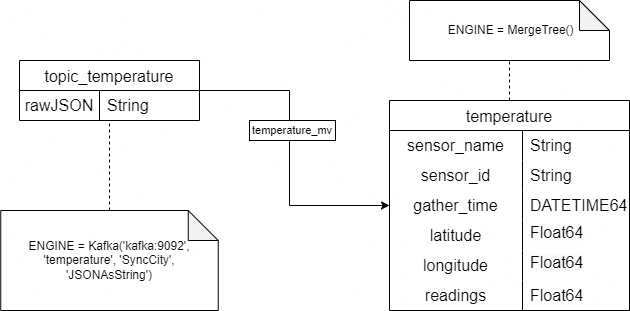
\includegraphics[width=0.8\textwidth]{images_st/tabelle_temperature.png}
    \caption{Schema tabelle di tipo temperature.}
    \label{fig:Schema tabelle di tipo temperature}
\end{figure}
\clearpage
\subsubsection{Sensore di umidità}
Nella tabella per i sensori di umidità viene salvato in ``readings" il valore di umidità generato.
\begin{figure}[h!]
    \centering
    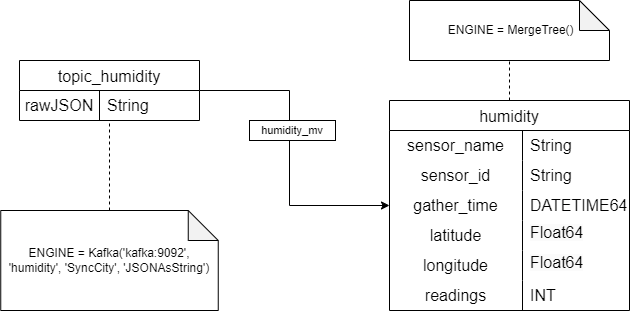
\includegraphics[width=0.8\textwidth]{images_st/tabelle_humidity.png}
    \caption{Schema tabelle di tipo humidity.}
    \label{fig:Schema tabelle di tipo humidity}
\end{figure}
\subsubsection{Sensore di intensità di precipitazione}
Nella tabella per i sensori di intensità di precipitazione viene salvato in ``readings" il valore di intensità generato.
\begin{figure}[h!]
    \centering
    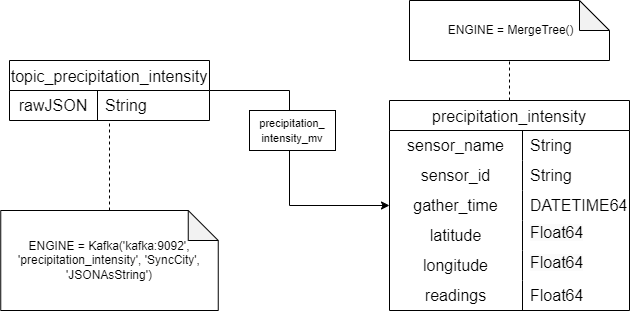
\includegraphics[width=0.8\textwidth]{images_st/tabelle_precipitation_intensity.png}
    \caption{Schema tabelle di tipo precipitation\_intensity.}
    \label{fig:Schema tabelle di tipo precipitation_intensity}
\end{figure}
\clearpage
\subsubsection{Sensore di inquinamento dell'aria}
Nella tabella per i sensori di inquinamento dell'aria vengono salvati i valori di inquinamento dovuto al particolato, all'ozono e al diossido di azoto nelle chiavi ``PM2\_5", ``PM10", ``O3" e ``NO2".
\begin{figure}[h!]
    \centering
    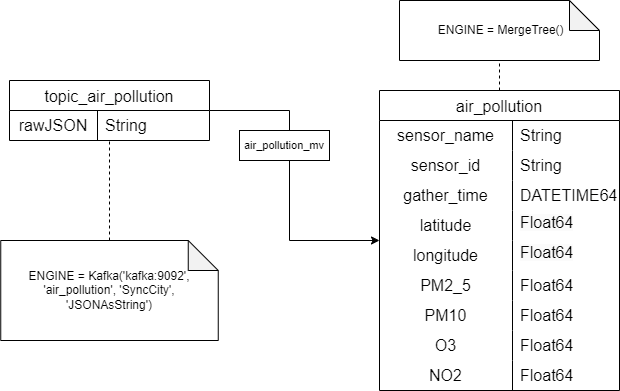
\includegraphics[width=0.8\textwidth]{images_st/tabelle_air_pollution.png}
    \caption{Schema tabelle di tipo air\_pollution.}
    \label{fig:Schema tabelle di tipo air_pollution}
\end{figure}
\subsubsection{Sensore di misurazione del livello dell'acqua}
Nella tabella per i sensori di misurazione del livello dell'acqua viene salvato in ``readings" il valore del livello dell'acqua generato.
\begin{figure}[h!]
    \centering
    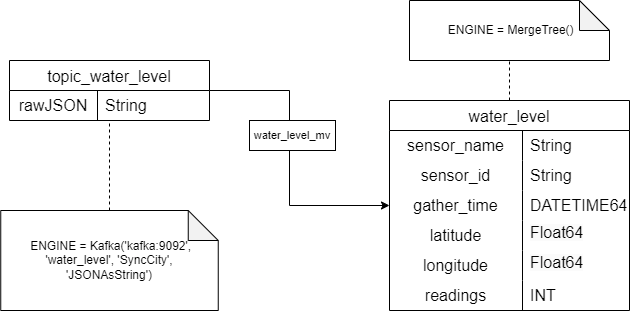
\includegraphics[width=0.8\textwidth]{images_st/tabelle_water_level.png}
    \caption{Schema tabelle di tipo water\_level.}
    \label{fig:Schema tabelle di tipo water_level}
\end{figure}
\clearpage
\subsubsection{Sensore di occupazione di parcheggi}
Nella tabella per i sensori di occupazione dei parcheggi vengono salvati lo stato di occupazione, la targa dell'occupante e il tempo di permanenza nelle chiavi ``is\_available", ``plate" e ``layoff".
\begin{figure}[h!]
    \centering
    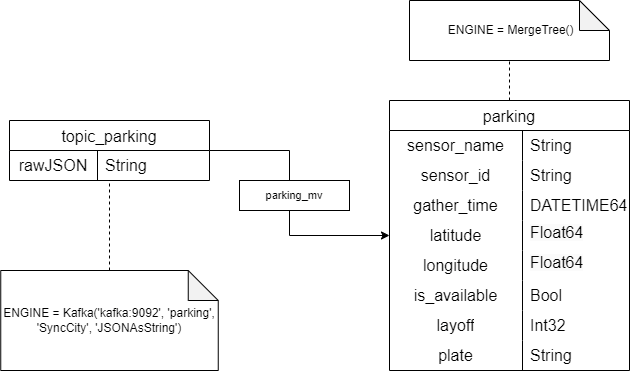
\includegraphics[width=0.8\textwidth]{images_st/tabelle_parking.png}
    \caption{Schema tabelle di tipo parking.}
    \label{fig:Schema tabelle di tipo parking}
\end{figure}
\subsubsection{Sensore di pagamento dei parcheggi}
Nella tabella per i sensori di pagamento dei parcheggi viene salvato in ``bill" l'importo del pagamento generato.
\begin{figure}[h!]
    \centering
    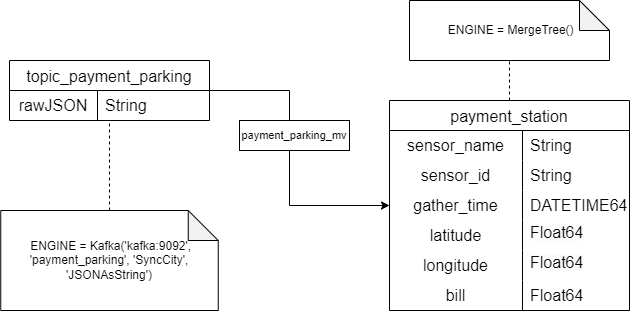
\includegraphics[width=0.8\textwidth]{images_st/tabelle_payment_parking.png}
    \caption{Schema tabelle di tipo payment\_parking.}
    \label{fig:Schema tabelle di tipo payment_parking}
\end{figure}
\clearpage
\subsubsection{Sensore di guasto elettrico}
Nella tabella per i sensori di guasto elettrico vengono salvati lo stato di salute, il momento di occorrenza di un guasto e il tempo di riparazione nelle chiavi ``is\_ok", ``occurence\_fault" e ``repair\_time".
\begin{figure}[h!]
    \centering
    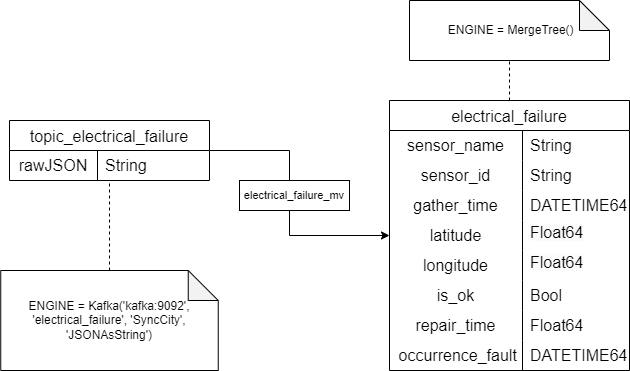
\includegraphics[width=0.8\textwidth]{images_st/tabelle_electrical_failure.png}
    \caption{Schema tabelle di tipo electrical\_failure.}
    \label{fig:Schema tabelle di tipo electrical_failure}
\end{figure}
\subsubsection{Sensore di riempimento isole ecologiche}
Nella tabella per i sensori di riempimento delle isole ecologiche viene salvato in ``readings" il valore di rimepimento generato.
\begin{figure}[h!]
    \centering
    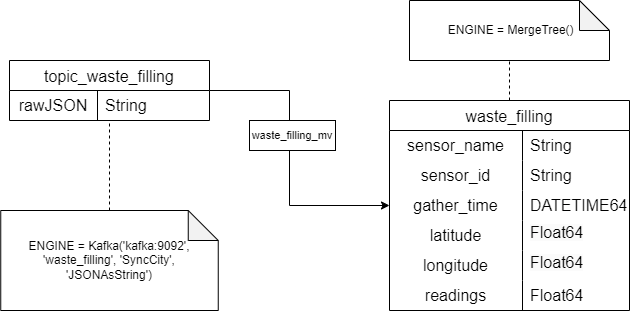
\includegraphics[width=0.8\textwidth]{images_st/tabelle_waste_filling.png}
    \caption{Schema tabelle di tipo waste\_filling.}
    \label{fig:Schema tabelle di tipo waste_filling}
\end{figure}
\clearpage
\subsubsection{Sensore di occupazione delle colonnine di ricarica}
Nella tabella per i sensori di occupazione delle colonnine di ricarica vengono salvati lo stato di occupazione, la targa dell'occupante e il tempo di permanenza nelle chiavi ``is\_available", ``plate" e ``layoff".
\begin{figure}[h!]
    \centering
    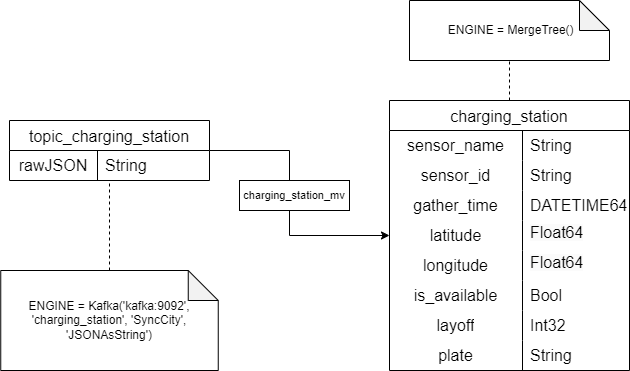
\includegraphics[width=0.8\textwidth]{images_st/tabelle_charging_station.png}
    \caption{Schema tabelle di tipo charging\_station.}
    \label{fig:Schema tabelle di tipo charging_station}
\end{figure}
\subsubsection{Sensore di pagamento delle colonnine di ricarica}
Nella tabella per i sensori di pagamento delle colonnine di ricarica viene salvato in ``bill" l'importo del pagamento generato.
\begin{figure}[h!]
    \centering
    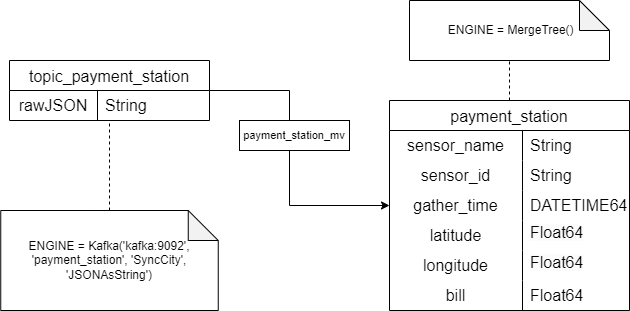
\includegraphics[width=0.8\textwidth]{images_st/tabelle_payment_station.png}
    \caption{Schema tabelle di tipo payment\_station.}
    \label{fig:Schema tabelle di tipo payment_station}
\end{figure}
\clearpage
\subsubsection{Sensore di consumo delle colonnine di ricarica}
Nella tabella per i sensori di consumo delle colonnine di ricarica viene salvato in ``kwh" il valore di consumo generato.
\begin{figure}[h!]
    \centering
    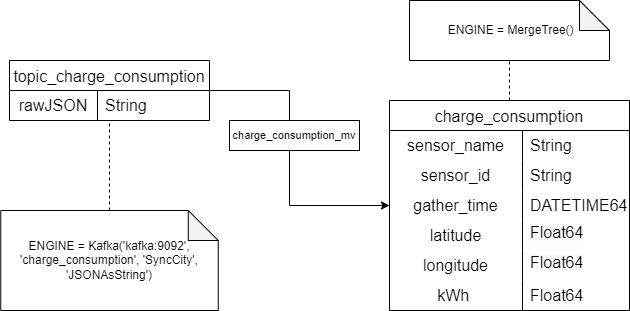
\includegraphics[width=0.8\textwidth]{images_st/tabelle_charge_consumption.png}
    \caption{Schema tabelle di tipo charge\_consumption.}
    \label{fig:Schema tabelle di tipo charge_consumption}
\end{figure}
\subsubsection{Calcolo della temperatura percepita}
Il calcolo della temperatura percepita avviene attraverso stream processing, elaborando gli stream di temperatura e di umidità. Lo stream uscente è poi passato a \glossterm{Kafka} come nuovo e dedicato topic e possiede quindi una sua tabella specifica. Il valore di temperatura percepita calcolato è salvato in ``readings".
\begin{figure}[h!]
    \centering
    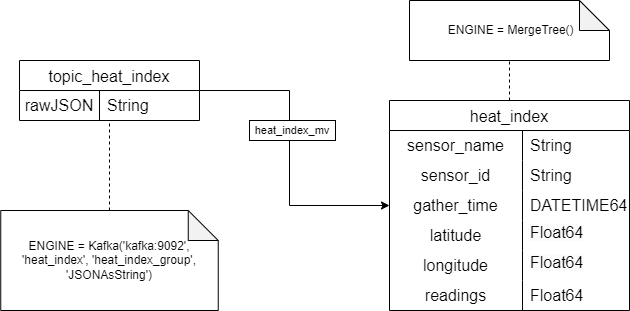
\includegraphics[width=0.8\textwidth]{images_st/tabelle_heat_index.png}
    \caption{Schema tabelle di tipo heat\_index.}
    \label{fig:Schema tabelle di tipo heat_index}
\end{figure}
\clearpage
\subsubsection{Calcolo dell'efficienza dei parcheggi}
Il calcolo dell'efficienza dei parcheggi avviene attraverso stream processing, elaborando gli stream di occupazione e pagamento dei parcheggi. Lo stream uscente è poi passato a \glossterm{Kafka} come nuovo e dedicato topic e possiede quindi una sua tabella specifica. Il valore di efficienza calcolato è salvato in ``readings".
\begin{figure}[h!]
    \centering
    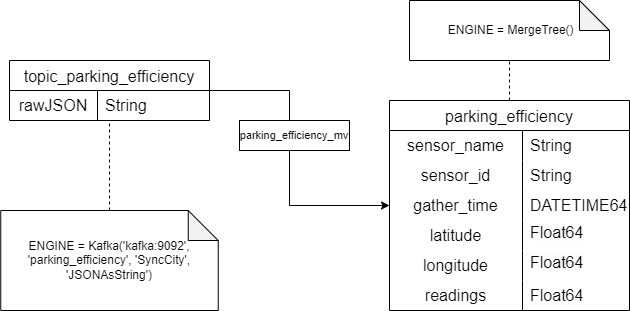
\includegraphics[width=0.8\textwidth]{images_st/tabelle_parking_efficiency.png}
    \caption{Schema tabelle di tipo parking\_efficiency.}
    \label{fig:Schema tabelle di tipo parking_efficiency}
\end{figure}
\subsection{\glossterm{Grafana}}
\glossterm{Grafana} permette la creazione di svariati tipi di \glossterm{dashboard} e \glossterm{widget} per la rappresentazione grafica dei dati simulati. L'utilizzo di tali dashboard è schermato dalla necessità di autenticarsi attarverso le credenziali fornite dall'amministratore di \glossterm{sistema}.
\subsubsection{User}
L’accesso a Grafana è vincolato a due utenze:
\begin{itemize}
    \item Amministratore di \glossterm{sistema}: 
    \begin{itemize}
        \item Manutenzione e modifiche della piattaforma;
        \item Non accessibile in produzione;
        \item Credenziali:
        \begin{itemize}
            \item \textbf{Username:} admin
            \item \textbf{Password:} admin
        \end{itemize}
    \end{itemize}
    \item User: 
    \begin{itemize}
        \item Amministratore pubblico o autorità locale per la visualizzazione e il monitoraggio dei dati;
        \item Credenziali:
        \begin{itemize}
            \item \textbf{Username:} user
            \item \textbf{Password:} user
        \end{itemize}
    \end{itemize}
\end{itemize}
\subsubsection{Datasource}
Come sorgente dati è stato impostato un collegamento con il database \glossterm{ClickHouse} grazie ad un plug-in installato attraverso file yaml di configurazione presente in ``/provisioning/datasources". Questo plugin di grafana consente di connettersi a un’istanza di ClickHous, di visualizzarne i dati in tempo reale ed eseguire query personalizzate.
\subsubsection{Dashboard}
I dati rappresentati sono stati categorizzati in base alla tipologia di informazione che forniscono. Sono stati individuati due ambiti:
\begin{itemize}
    \item \textbf{Dati ambientali:} Dati che forniscono informazioni riguardanti il clima e l'ambiente;
    \item \textbf{Dati urbanistici:} Dati che forniscono informazioni riguardanti lo stato dei servizi urbanistici nella città.
\end{itemize}
Le \glossterm{dashboard} implementate sono quattro.
\subsubsubsection{Sensors} 
\glossterm{Dashboard} riguardante informazioni generiche sui sensori. Questa dashboard si compone del seguente pannello:
\begin{itemize}
    \item Pannello \glossterm{geomap} per la visualizzazione della locazione geografica dei sensori.
\end{itemize}
\subsubsubsection{Environmental planning} 
\glossterm{Dashboard} riguardante le informazioni di tipo ambientale.
Ai fini di una migliore organizzazione dei dati visualizzati e di una più efficace comprensione dei pannelli visualizzati, quest'ultimi sono suddivisi compartimenti attraverso righe comprimibili.
\begin{itemize}
    \item \textbf{Riga Temperature:}
    \begin{itemize}
        \item Pannello \glossterm{time-series} per il monitoraggio dell'andamento della temperatura;
        \item Pannello \glossterm{Gauge} per il valore medio di temperatura misurata;
        \item Pannello a barre per valori statistici, quali media, moda, minimo e massimo di temperatura rilevata.
    \end{itemize}
    \item \textbf{Riga Heat Index:}
    \begin{itemize}
        \item Pannello \glossterm{time-series} per il monitoraggio dell'andamento della temperatura percepita;
        \item Pannello \glossterm{Gauge} per il valore medio di temperatura percepita;
        \item Pannello a barre per valori statistici, quali media, minimo e massimo di temperatura percepita.
    \end{itemize}
    \item \textbf{Riga Humidity:}
    \begin{itemize}
        \item Pannello \glossterm{time-series} per il monitoraggio dell'andamento dell'umidità;
        \item Pannello \glossterm{Gauge} per il valore medio di umidità misurata.
    \end{itemize}
    \item \textbf{Riga Precipitation Intensity:}
    \begin{itemize}
        \item Pannello \glossterm{time-series} per il monitoraggio dell'andamento dell'intensità di precipitazione;
        \item Pannello \glossterm{Gauge} per il valore medio di intensità di precipitazione misurata.
    \end{itemize}
    \item \textbf{Riga Air Pollution:}
    \begin{itemize}
        \item Pannello \glossterm{time-series} per il monitoraggio dell'andamento dei valori di inquinamento dell'aria PM2.5, PM10, O3 e NO2;
        \item Pannello \glossterm{time-series} per il monitoraggio dell'andamento della quantità di PM2.5 nell'aria;
        \item Pannello \glossterm{time-series} per il monitoraggio dell'andamento della quantità di PM10 nell'aria;
        \item Pannello \glossterm{time-series} per il monitoraggio dell'andamento della quantità di O3 nell'aria;
        \item Pannello \glossterm{time-series} per il monitoraggio dell'andamento della quantità di NO2 nell'aria;
        \item Pannello \glossterm{Gauge} per il valore medio di PM2.5 misurato;
        \item Pannello \glossterm{Gauge} per il valore medio di PM10 misurato;
        \item Pannello \glossterm{Gauge} per il valore medio di O3 misurato;
        \item Pannello \glossterm{Gauge} per il valore medio di NO2 misurato.
    \end{itemize}
    \item \textbf{Riga Water Level:}
    \begin{itemize}
        \item Pannello \glossterm{time-series} per il monitoraggio dell'andamento del livello dell'acqua;
        \item Pannello \glossterm{Gauge} per il valore medio del livello dell'acqua misurato. 
    \end{itemize}
\end{itemize}
\subsubsubsection{Urban planning} 
\glossterm{Dashboard} riguardante le informazioni di tipo urbanistico.
Ai fini di una migliore organizzazione dei dati visualizzati e di una più efficace comprensione dei pannelli visualizzati, quest'ultimi sono suddivisi compartimenti attraverso righe comprimibili.
\begin{itemize}
    \item \textbf{Riga Parking:}
    \begin{itemize}
        \item Pannello \glossterm{geomap} per il monitoraggio della percentuale di occupazione di un parcheggio;
        \item Pannello in formato tabellare per tracciare l'occupazione e valutare la disponibilità dei singoli stalli;
        \item Pannello a barre per valori statistici, quali media, minimo e massimo pagamento effettuato per l'utilizzo di uno stallo di parcheggio;
        \item Pannello in formato di registro per segnalare i pagamaneti effettuati per l'utilizzo degli stalli di parcheggio;
        \item Pannello \glossterm{Gauge} per il valore di efficienza di un parcheggio.
    \end{itemize}
    \item \textbf{Riga Charging Stations:}
    \begin{itemize}
        \item Pannello \glossterm{geomap} per il monitoraggio della percentuale di occupazione delle colonnine di ricarica;
        \item Pannello in formato tabellare per tracciare l'occupazione e valutare la disponibilità delle colonnine di ricarica;
        \item Pannello a barre per valori statistici, quali media, minimo e massimo pagamento effettuato per l'utilizzo di una colonnina di ricarica;
        \item Pannello in formato di registro per segnalare i pagamaneti effettuati per l'utilizzo delle colonnine di ricarica;
        \item Pannello \glossterm{time-series} per il monitoraggio dei consumi delle colonnine di ricarica;
    \end{itemize}
    \item \textbf{Riga Waste Fill:}
    \begin{itemize}
        \item Pannello \glossterm{time-series} per il monitoraggio del riempimento delle isole ecologiche.
    \end{itemize}
    \item \textbf{Riga Electrical Failure:}
    \begin{itemize}
        \item Pannello \glossterm{geomap} per il monitoraggio dello stato di salute della linea elettrica.
    \end{itemize}
\end{itemize}
\subsubsubsection{Exceeding Thresholds}
Quest'ultima \glossterm{dashboard} si concentra sulla visualizzazione degli alert attivi. I pannelli sono divisi in due categorie:
\begin{itemize}
    \item \textbf{Riga Environmental Planning:}
    \begin{itemize}
        \item Pannello \glossterm{alertlist} per tracciare lo stato degli alert relativi alla temperatura percepita;
        \item Pannello \glossterm{alertlist} per tracciare lo stato degli alert relativi all'intensità di precipitazione;
        \item Pannello \glossterm{alertlist} per tracciare lo stato degli alert relativi all'inquinamento dell'aria da PM10;
        \item Pannello \glossterm{alertlist} per tracciare lo stato degli alert relativi al livello dell'acqua.
    \end{itemize}
    \item \textbf{Riga Urban Planning:}
    \begin{itemize}
        \item Pannello \glossterm{alertlist} per tracciare lo stato degli alert relativi al riempimento delle isole ecologiche.
    \end{itemize}
\end{itemize}
\subsubsection{Variables}
Le variabili in \glossterm{Grafana} rendono le \glossterm{dashboard} dinamiche e
interattive. Grazie a valori scelti dall'utente permettono di visualizzare dati provenienti da sensori diversi operando da filtro ma anche da metodo di confronto tra sensori dello stesso tipo.
\\Le variabili nel progetto sono state implementate attraverso i file di provisioning. Nello specifico, nei file \glossterm{JSON} che descrivono le dashboard è possibile definire i valori che le variabili nei \glossterm{widget} possono assumere.
\\Le variabili utilizzate riguardano unicamente lo specifico sensore analizzato per tipologia: un tipo di sensore può quindi confrontare nello stesso pannello tutti i sensori della stessa tipologia o concentrarsi nel monitoraggio di uno in particolare. Questo aumenta la versatilità di utilizzo delle dashboard.
\subsubsection{Alerts}
\glossterm{Grafana} offre un \glossterm{sistema} di notifica per avvisare della presenza di anomalie nei dati quando si verificano determinate condizioni. Le notifiche possono essere inviate tramite diversi canali, tra cui email, \glossterm{Telegram} e \glossterm{Discord}.
\\La configurazione di un alert avviene impostando una alert rule tramite query. L’alert si attiva quando la condizione impostata viene soddisfatta. Gli alert sono configurati per i seguenti eventi:
\begin{itemize}
    \item Quando un sensore di temperatura segnala una temperatura superiore ai 40°C  inferiore ai -10°C;
    \item Quando un sensore di intensità di precipitazione segnala un'intensità superiore ai 30 mm/h;
    \item Quando un sensore di inquinamento dell'aria segnala un valore di inquinamento da PM10 superiore a 80 µg / $\mbox{m}^{\mbox{3}}$;
    \item Quando un sensore di rilevazione del livello dell'acqua segnala un livello superiore a 80\% della capacità del bacino;
    \item Quando un sensore di riempimento delle isole ecologiche segnala un riempimento superiore a 80\% della capacità del conferitore;
\end{itemize}
Gli alert possono trovarsi i quattro stati:
\begin{itemize}
    \item \textbf{No data:} Non ci sono dati in arrivo dal database;
    \item \textbf{Error:} Ci sono errori nei dati o nelle query dei pannelli;
    \item \textbf{Normal:} Indica che un alert è disattivato e la condizione di alert non è soddisfatta.
    \item \textbf{Pending:}Indica che la condizione per l’attivazione dell’alert è stata soddisfatta, ma non è ancora trascorso il periodo di valutazione;
    \item \textbf{Firing:} Indica che un alert è stato attivato, la condizione di alert è stata soddisfatta per il periodo di valutazione definito. Viene quindi inviata una notifica ai canali impostati.
\end{itemize}
Le regole sono configurabili tramite l’interfaccia grafica successivamente inserite in formato yaml in ``/provisioning/alerting".
\subsubsection{Canali di notifica}
La configurazione dei canali di notifica avviene da interfaccia grafica nella sezione ``Alerting/Notification channels".
È stato scelto \glossterm{Discord} come unico canale di notifica.
Per configurare Discord come canale di notifica è necessario:
\begin{itemize}
    \item Selezionare Discord;
    \item Configurare il server Discord ``SyncCity";
    \item Ottenere il webhook URL del canale in: ``Impostazioni server/Integrazioni" e selezionare ``Visualizza webhook";
    \item Inserire il webhook URL del canale;
    \item Personalizzare il messaggio di notifica.
\end{itemize}
Le impostazioni di configurazione del canale di notifica sono esportabili in formato yaml e inseribili in ``/provisioning/alerting".
\newpage
\section{Architettura di deployment}\label{sec:dep}
L’intero stack tecnologico è stato implementato e configurato attraverso un ambiente \glossterm{Docker} che ha permesso lo sviluppo del modello a layer precedentemente descritto e dei suoi servizi. I container che verranno descritti sono presenti nel file \textit{docker-compose.yaml} nella \glossterm{repository} del team.
\subsection{Data source}
La sorgente dati presenta due container:
\begin{itemize}
    \item \textbf{Container pymocksensors:}
    \begin{itemize}
        \item Esegue il generatore dati;
        \item Utilizzato per la produzione dei messaggi \glossterm{JSON} indirizzati allo streaming layer.
    \end{itemize}
    \item \textbf{Container pymocksensors-test:}
        \item Esegue i test d'unità e d'integrazione.
\end{itemize}
\subsection{Streaming layer}
\begin{itemize}
    \item \textbf{Container kafka:}
    \begin{itemize}
        \item Esegue \glossterm{Kafka} per la gestione del flusso dei dati;
        \item Utilizzato in produzione dati, per i test d'integrazione e per il testing dello stream processing;
        \item Accessibile agli altri container attraverso l'indirizo \textit{kafka:9092}.
    \end{itemize}
\end{itemize}
\subsection{Processing layer}
\begin{itemize}
    \item \textbf{Container jobmanager:}
    \begin{itemize}
        \item Gestisce i job e quindi le task per l'elaborazione degli stream dati.
    \end{itemize}
    \item \textbf{Container taskmanager:}
    \begin{itemize}
        \item Gestisce le operazioni di stream processing definite.
    \end{itemize}
    \item \textbf{Container flink-deployer:}
    \begin{itemize}
        \item Esegue \glossterm{Flink} e in particolare provvede al funzionamento del jobmanager e del taskmanager.
    \end{itemize}
\end{itemize}
\subsection{Storage layer}
\begin{itemize}
    \item \textbf{Container clickhouse:}
    \begin{itemize}
        \item Esegue \glossterm{ClickHouse} per l'archiviazione dei dati;
        \item Accessibile agli altri container attraverso l'indirizzo \textit{clickhouse:8123}.
    \end{itemize}
\end{itemize}
\subsection{Visualization layer}
\begin{itemize}
    \item \textbf{Container grafana:}
    \begin{itemize}
        \item Esegue \glossterm{Grafana} per la visualizzazione dei dati;
        \item Accessibile all'esterno nel browser all'indirizzo \textit{localhost:3000}.
    \end{itemize}
\end{itemize}
\newpage
\section{Tracciamento requisiti}\label{sec:trac}
Di seguito è riportato, per ogni requisito, il corrispondente codice, secondo la tabella presente nel documento \textit{Analisi dei Requisiti v2.0.0}, la sua descrizione e se tale requisito è stato soddisfatto.
\newcounter{row}
\setcounter{row}{0}
\newcommand{\rownumber}{\stepcounter{row}\arabic{row}}
\renewcommand{\arraystretch}{2.5}
\rowcolors{2}{gray!20}{white}
\begin{longtable}{|>{\centering\arraybackslash}p{1.2cm}|>{\centering\arraybackslash}p{2cm}|>{\centering\arraybackslash}p{8.5cm}|>{\centering\arraybackslash}p{3cm}|}
    \hline
    \rowcolor{white}
	\textbf{Codice} & \textbf{Importanza} & \textbf{Descrizione} & \textbf{Stato}\\ \hline
 \endfirsthead
 \rowcolor{white}
    \caption{Requisiti funzionali.}
	\label{table:Requisiti funzionali}
 \endlastfoot
            RF-\rownumber & Obbligatorio & L'utente deve effettuare l'autenticazione per poter usufruire del \glossterm{sistema}. Le credenziali di accesso sono fornite dall'amministratore del \glossterm{sistema}. & Soddisfatto \\ \hline
            RF-\rownumber & Obbligatorio & Il \glossterm{sistema} deve permettere la visualizzazione in tempo reale dei dati provenienti dai sensori. & Soddisfatto \\ \hline 
            RF-\rownumber & Obbligatorio & Il \glossterm{sistema} deve integrare molteplici simulatori di sensori in grado di generare dati casuali ma comunque verosimili. & Soddisfatto \\ \hline
            RF-\rownumber & Obbligatorio & Il \glossterm{sistema} deve integrare almeno un \glossterm{sensore} che rilevi la temperatura, espressa in gradi Celsius. & Soddisfatto \\ \hline
            RF-\rownumber & Obbligatorio & Il \glossterm{sistema} deve integrare almeno un \glossterm{sensore} che rilevi l'umidità nell'aria, espressa in percentuale. & Soddisfatto \\ \hline
            RF-\rownumber & Obbligatorio & Il \glossterm{sistema} deve integrare almeno un \glossterm{sensore} che rilevi l'intensità delle precipitazioni, espressa in millimetri orari. & Soddisfatto \\ \hline
            RF-\rownumber & Obbligatorio & Il \glossterm{sistema} deve integrare almeno un \glossterm{sensore} che rilevi la quantità di polveri sottili presenti nell'aria, espressa in microgrammi per metro cubo. & Soddisfatto \\ \hline
            RF-\rownumber & Obbligatorio & Il \glossterm{sistema} deve integrare almeno un \glossterm{sensore} che rilevi il livello dell'acqua nella zona di installazione, espresso in percentuale. & Soddisfatto \\ \hline
            RF-\rownumber & Obbligatorio & Il \glossterm{sistema} deve integrare almeno un \glossterm{sensore} che rilevi lo stato di occupazione dei parcheggi, espresso mediante un valore binario. & Soddisfatto \\ \hline    
            RF-\rownumber & Obbligatorio & Il \glossterm{sistema} deve integrare almeno un \glossterm{sensore} che invii dati di pagamento per parcheggi. & Soddisfatto \\ \hline
            RF-\rownumber & Obbligatorio & Il \glossterm{sistema} deve integrare almeno un \glossterm{sensore} che rilevi la presenza di guasti elettrici, espressa mediante un valore binario. & Soddisfatto \\ \hline
            RF-\rownumber & Obbligatorio & Il \glossterm{sistema} deve integrare almeno un \glossterm{sensore} che rilevi lo stato di riempimento delle isole ecologiche, espresso mediante un valore binario. & Soddisfatto \\ \hline
            RF-\rownumber & Obbligatorio & Il \glossterm{sistema} deve integrare almeno un \glossterm{sensore} che rilevi lo stato di utilizzo delle colonnine di ricarica, espresso mediante un valore binario. & Soddisfatto \\ \hline
            RF-\rownumber & Obbligatorio & Il \glossterm{sistema} deve integrare almeno un \glossterm{sensore} che rilevi il consumo di energia delle colonnine di ricarica. & Soddisfatto \\ \hline
            RF-\rownumber & Obbligatorio & Il \glossterm{sistema} deve integrare almeno un \glossterm{sensore} che invii dati di pagamento per colonnine di ricarica. & Soddisfatto \\ \hline
            RF-\rownumber & Obbligatorio & L'utente deve poter digitare il proprio username nel campo di inserimento corrispondente per accedere al \glossterm{sistema}. & Soddisfatto \\ \hline
            RF-\rownumber & Obbligatorio & L'utente deve poter digitare la propria password nel campo di inserimento corrispondente per accedere al \glossterm{sistema}. & Soddisfatto \\ \hline
            RF-\rownumber & Obbligatorio & L'utente deve poter visualizzare un messaggio di errore qualora le credenziali di accesso inserite fossero errate. & Soddisfatto \\ \hline
            RF-\rownumber & Obbligatorio & L'utente deve poter visualizzare un menu attraverso il quale selezionare la \glossterm{dashboard} desiderata tra Sensori, Ambientale ed Urbanistica. & Soddisfatto \\ \hline
            RF-\rownumber & Obbligatorio & L'utente deve poter visualizzare la \glossterm{dashboard} relativa allo stato dei sensori. & Soddisfatto \\ \hline
            RF-\rownumber & Obbligatorio & L'utente deve poter visualizzare un \glossterm{widget} contente una mappa su cui è indicata la posizione geografica dei sensori. & Soddisfatto \\ \hline
            RF-\rownumber & Obbligatorio & L'utente deve poter visualizzare il nome e le coordinate geografiche dei singoli sensori collocati all'interno del territorio urbano. & Soddisfatto \\ \hline
            RF-\rownumber & Obbligatorio & L'utente deve poter visualizzare la \glossterm{dashboard} relativa al dominio ambientale. & Soddisfatto \\ \hline
            RF-\rownumber & Obbligatorio & L'utente deve poter visualizzare un \glossterm{widget} che mostra le rilevazioni della temperatura in formato \glossterm{time series}. & Soddisfatto \\ \hline
            RF-\rownumber & Obbligatorio & L'utente deve poter visualizzare un \glossterm{widget} che mostra le rilevazioni dell'umidità in formato \glossterm{time series}. & Soddisfatto \\ \hline
            RF-\rownumber & Desiderabile & L'utente deve poter visualizzare un \glossterm{widget} che mostra le rilevazioni della temperatura percepita in formato \glossterm{time series}. & Soddisfatto \\ \hline
            RF-\rownumber & Desiderabile & L'utente deve poter visualizzare un \glossterm{widget} che mostra la temperatura media in formato diagramma di \glossterm{Gauge} considerando le ultime rilevazioni effettuate dai singoli sensori attivi. & Soddisfatto \\ \hline
            RF-\rownumber & Desiderabile & L'utente deve poter visualizzare un \glossterm{widget} che mostra l'umidità media in formato diagramma di \glossterm{Gauge} considerando le ultime rilevazioni effettuate dai singoli sensori attivi. & Soddisfatto \\ \hline
            RF-\rownumber & Desiderabile & L'utente deve poter visualizzare un \glossterm{widget} che mostra la temperatura percepita media in formato diagramma di \glossterm{Gauge} considerando le ultime rilevazioni effettuate dalle coppie di sensori temperatura-umidità attivi. & Soddisfatto \\ \hline
            RF-\rownumber & Desiderabile & L'utente deve poter visualizzare un \glossterm{widget} che mostra le statistiche di temperatura in formato diagramma a barre considerando ciascun \glossterm{sensore} attivo nell'intervallo di tempo. & Soddisfatto \\ \hline
            RF-\rownumber & Desiderabile & L'utente deve poter visualizzare un \glossterm{widget} che mostra le statistiche di temperatura percepita in formato diagramma a barre considerando ciascuna coppia di valori di temperatura e umidità per ogni rispettivo \glossterm{sensore} attivo nell'intervallo di tempo. & Soddisfatto \\ \hline
            RF-\rownumber & Obbligatorio & L'utente deve poter visualizzare un \glossterm{widget} che mostra l'intensità delle precipitazioni in formato \glossterm{time series}. & Soddisfatto \\ \hline
            RF-\rownumber & Obbligatorio & L'utente deve poter visualizzare un \glossterm{widget} che mostra l'inquinamento dell'aria in formato \glossterm{time series}. & Soddisfatto \\ \hline
            RF-\rownumber & Obbligatorio & L'utente deve poter visualizzare un \glossterm{widget} che mostra il livello dell'acqua in formato \glossterm{time series}. & Soddisfatto \\ \hline
            RF-\rownumber & Desiderabile & L'utente deve poter visualizzare un \glossterm{widget} che mostra l'intensità attuale delle precipitazioni in formato diagramma di \glossterm{Gauge} considerando le ultime rilevazioni effettuate dai singoli sensori attivi. & Soddisfatto \\ \hline
            RF-\rownumber & Desiderabile & L'utente deve poter visualizzare un \glossterm{widget} che mostra l'inquinamento attuale dell'aria in formato diagramma di \glossterm{Gauge} considerando le ultime rilevazioni effettuate dai singoli sensori attivi. & Soddisfatto \\ \hline
            RF-\rownumber & Desiderabile & L'utente deve poter visualizzare un \glossterm{widget} che mostra il livello attuale dell'acqua in formato diagramma di \glossterm{Gauge} considerando le ultime rilevazioni effettuate dai singoli sensori attivi. & Soddisfatto \\ \hline
            RF-\rownumber & Obbligatorio & L'utente deve poter visualizzare la \glossterm{dashboard} relativa al dominio urbanistico. &Soddisfatto \\ \hline
            RF-\rownumber & Obbligatorio & L'utente deve poter visualizzare un \glossterm{widget} che mostra una mappa che descrive lo stato di occupazione dei parcheggi. & Soddisfatto \\ \hline
            RF-\rownumber & Obbligatorio & L'utente deve poter visualizzare un \glossterm{widget} che mostra una tabella che descrive i parcheggi. & Soddisfatto \\ \hline
            RF-\rownumber & Obbligatorio & L'utente deve poter visualizzare un \glossterm{widget} che mostra una lista di notifiche dei pagamenti dei parcheggi. & Soddisfatto \\ \hline
            RF-\rownumber & Obbligatorio & L'utente deve poter visualizzare un \glossterm{widget} che mostra una tabella che descrive i guasti alla fornitura elettrica. & Soddisfatto \\ \hline
            RF-\rownumber & Obbligatorio & L'utente deve poter visualizzare un \glossterm{widget} che mostra lo stato di riempimento delle isole ecologiche in formato \glossterm{time series}. & Soddisfatto \\ \hline
            RF-\rownumber & Obbligatorio & L'utente deve poter visualizzare un \glossterm{widget} che mostra una mappa che descrive la disponibilità colonnine di ricarica. & Soddisfatto \\ \hline
            RF-\rownumber & Obbligatorio & L'utente deve poter visualizzare un \glossterm{widget} che mostra una tabella che le colonnine di ricarica. & Soddisfatto \\ \hline
            RF-\rownumber & Desiderabile & L'utente deve poter visualizzare un \glossterm{widget} che mostra i consumi di elettricità delle colonnine di ricarica in formato \glossterm{time series}. & Soddisfatto \\ \hline
            RF-\rownumber & Obbligatorio & L'utente deve poter visualizzare un \glossterm{widget} che mostra le notifiche di pagamento relative all'utilizzo delle colonnine di ricarica. & Soddisfatto \\ \hline
            RF-\rownumber & Obbligatorio & L'utente deve poter visualizzare un \glossterm{widget} che mostra le statistiche relative ai pagamenti dovuti a parcheggi. & Soddisfatto \\ \hline
            RF-\rownumber & Obbligatorio & L'utente deve poter visualizzare un \glossterm{widget} che mostra le statistiche relative ai pagamenti dovuti a colonnine di ricarica. & Soddisfatto \\ \hline
            RF-\rownumber & Obbligatorio & L'utente deve poter visualizzare un \glossterm{widget} che mostra l'efficienza monetaria dei parcheggi. & Soddisfatto \\ \hline
            RF-\rownumber & Desiderabile & L'utente deve poter visualizzare la \glossterm{dashboard} relativa al superamento delle soglie. & Soddisfatto \\ \hline
            RF-\rownumber & Desiderabile & L'utente deve poter visualizzare un \glossterm{widget} che mostra che mostra una lista di notifiche riguardanti il superamento delle soglie di temperatura. & Soddisfatto \\ \hline
            RF-\rownumber & Desiderabile & L'utente deve poter visualizzare un \glossterm{widget} che mostra che mostra una lista di notifiche riguardanti il superamento della soglia di precipitazioni. & Soddisfatto \\ \hline
            RF-\rownumber & Desiderabile & L'utente deve poter visualizzare un \glossterm{widget} che mostra che mostra una lista di notifiche riguardanti il superamento della soglia di inquinamento dell'aria. & Soddisfatto \\ \hline
            RF-\rownumber & Desiderabile & L'utente deve poter visualizzare un \glossterm{widget} che mostra che mostra una lista di notifiche riguardanti il superamento della soglia di livello dell'acqua. & Soddisfatto \\ \hline
            RF-\rownumber & Desiderabile & L'utente deve poter visualizzare un \glossterm{widget} che mostra che mostra una lista di notifiche riguardanti il superamento della soglia di riempimento dei conferitori nelle isole ecologiche. & Soddisfatto \\ \hline
            RF-\rownumber & Obbligatorio & L'utente deve poter visualizzare un messaggio di errore qualora non sia possibile reperire i dati o vi sia un malfunzionamento nel \glossterm{sistema}. & Soddisfatto \\ \hline
            RF-\rownumber & Obbligatorio & L'utente deve poter applicare dei filtri per escludere alcuni dati dalla visualizzazione, secondo determinati criteri. &Soddisfatto \\ \hline 
            RF-\rownumber & Obbligatorio & L'utente deve poter applicare dei filtri per visualizzare solo i dati provenienti da alcune specifiche tipologie di sensori. & Soddisfatto \\ \hline
            RF-\rownumber & Obbligatorio & L'utente deve poter applicare dei filtri per visualizzare solo i dati misurati in un determinato intervallo temporale. & Soddisfatto \\ \hline
            RF-\rownumber & Obbligatorio & L'utente deve poter rimuovere i filtri applicati in precedenza in modo da non escludere alcun dato dalla visualizzazione. & Soddisfatto \\ \hline
            RF-\rownumber & Desiderabile & L'utente deve poter modificare il layout dei \glossterm{widget} a proprio piacimento. & Soddisfatto \\ \hline
            RF-\rownumber & Desiderabile & L'utente deve poter ridimensionare i \glossterm{widget} a proprio piacimento. & Soddisfatto \\ \hline
            RF-\rownumber & Desiderabile & L'utente deve poter spostare i \glossterm{widget} a proprio piacimento. & Soddisfatto \\ \hline
            RF-\rownumber & Obbligatorio & Il \glossterm{sensore} deve poter inviare i dati misurati, assieme al timestamp di rilevazione e alle proprie coordinate geografiche. & Soddisfatto \\ \hline
            RF-\rownumber & Obbligatorio & Il \glossterm{sensore} deve poter inviare i dati relativi alla temperatura, assieme al timestamp di rilevazione e alle proprie coordinate geografiche. & Soddisfatto \\ \hline
            RF-\rownumber & Obbligatorio & Il \glossterm{sensore} deve poter inviare i dati relativi all'umidità, assieme al timestamp di rilevazione e alle proprie coordinate geografiche. & Soddisfatto \\ \hline
            RF-\rownumber & Obbligatorio & Il \glossterm{sensore} deve poter inviare i dati relativi alle precipitazioni, assieme al timestamp di rilevazione e alle proprie coordinate geografiche. & Soddisfatto \\ \hline
            RF-\rownumber & Obbligatorio & Il \glossterm{sensore} deve poter inviare i dati relativi all'inquinamento atmosferico, assieme al timestamp di rilevazione e alle proprie coordinate geografiche. & Soddisfatto \\ \hline
            RF-\rownumber & Obbligatorio & Il \glossterm{sensore} deve poter inviare i dati relativi al livello dell'acqua, assieme al timestamp di rilevazione e alle proprie coordinate geografiche. & Soddisfatto \\ \hline
            RF-\rownumber & Obbligatorio & Il \glossterm{sensore} deve poter inviare i dati relativi allo stato di occupazione dei parcheggi, assieme al timestamp di rilevazione e alle proprie coordinate geografiche. & Soddisfatto \\ \hline
            RF-\rownumber & Obbligatorio & Il \glossterm{sensore} deve poter inviare i dati relativi ai pagamenti dei parcheggi, assieme al timestamp di rilevazione e alle proprie coordinate geografiche. & Soddisfatto \\ \hline
            RF-\rownumber & Obbligatorio & Il \glossterm{sensore} deve poter inviare i dati relativi ai guasti elettrici, assieme al timestamp di rilevazione e alle proprie coordinate geografiche. & Soddisfatto \\ \hline
            RF-\rownumber & Obbligatorio & Il \glossterm{sensore} deve poter inviare i dati relativi al livello di riempimento dei conferitori nelle isole ecologiche, assieme al timestamp di rilevazione e alle proprie coordinate geografiche. & Soddisfatto \\ \hline
            RF-\rownumber & Obbligatorio & Il \glossterm{sensore} deve poter inviare i dati relativi allo stato di occupazione delle colonnine di ricarica, assieme al timestamp di rilevazione e alle proprie coordinate geografiche. & Soddisfatto \\ \hline
            RF-\rownumber & Obbligatorio & Il \glossterm{sensore} deve poter inviare i dati relativi ai consumi di elettricità delle colonnine di ricarica, assieme al timestamp di rilevazione e alle proprie coordinate geografiche. & Soddisfatto \\ \hline
            RF-\rownumber & Obbligatorio & Il \glossterm{sensore} deve poter inviare i dati relativi ai pagamenti delle ricariche effettuate mediante colonnine elettriche, assieme al timestamp di rilevazione e alle proprie coordinate geografiche. & Soddisfatto \\ \hline
            RF-\rownumber & Obbligatorio & Il \glossterm{sistema} consentire la correlazione di dati provenienti da sensori diversi. & Soddisfatto \\ \hline
            RF-\rownumber & Opzionale & Il \glossterm{sistema} consentire la previsione di eventi futuri attraverso l'analisi dei dati provenienti dai sensori. & Non soddisfatto \\ \hline
\end{longtable}
\newpage
\rowcolors{2}{gray!20}{white}
\begin{longtable}{|>{\centering\arraybackslash}p{1.2cm}|>{\centering\arraybackslash}p{2cm}|>{\centering\arraybackslash}p{8.5cm}|>{\centering\arraybackslash}p{3cm}|}
    \hline
    \rowcolor{white}
    \textbf{Codice} & \textbf{Importanza} & \textbf{Descrizione} & \textbf{Stato} \\
    \hline
    \endfirsthead
    \rowcolor{white}
    \caption{Requisiti qualitativi.}
	\label{table:Requisiti qualitativi}
    \endlastfoot
            RQ-\rownumber & Obbligatorio & Devono essere rispettati i vincoli e le metriche descritti nel documento \textit{Piano di Qualifica v1.0.0}. & Soddisfatto \\ \hline
            RQ-\rownumber & Obbligatorio & Devono essere rispettate le norme specificate nel documento \textit{Norme di Progetto v1.0.0}. & Soddisfatto \\ \hline
            RQ-\rownumber & Obbligatorio & La copertura di test deve essere almeno dell'80\% e deve essere adeguatamente documentata. & Soddisfatto \\ \hline
            RQ-\rownumber & Obbligatorio & La \glossterm{Proponente} deve essere in grado di accedere alla \glossterm{repository} \glossterm{GitHub} del prodotto ``SyncCity''. & Soddisfatto \\ \hline
            RQ-\rownumber & Obbligatorio & Il corretto funzionamento dei simulatori di sensori deve essere adeguatamente documentato. Esso deve essere descritto in un documento aggiuntivo appositamente redatto. & Soddisfatto \\ \hline
            RQ-\rownumber & Obbligatorio & Le scelte implementative e progettuali devono essere motivate ed adeguatamente documentate. Esse dovranno essere descritte in un documento aggiuntivo appositamente redatto. & Soddisfatto \\ \hline
            RQ-\rownumber & Obbligatorio & I problemi aperti e le eventuali soluzioni da esplorare devono essere adeguatamente documentati. Essi dovranno essere descritti in un documento aggiuntivo appositamente redatto. & Soddisfatto \\ \hline
            RQ-\rownumber & Obbligatorio & Deve essere fornito il documento \textit{Manuale Utente} che illustra le funzionalità offerte dal \glossterm{sistema} e le modalità di fruizione delle stesse. & Soddisfatto \\ \hline
            RQ-\rownumber & Obbligatorio & Deve essere fornito il documento \textit{Specifica Tecnica} che illustra le scelte architetturali e progettuali effettuate. & Soddisfatto \\ \hline            
\end{longtable}
\newpage
\rowcolors{2}{gray!20}{white}
\begin{longtable}{|>{\centering\arraybackslash}p{1.2cm}|>{\centering\arraybackslash}p{2cm}|>{\centering\arraybackslash}p{8.5cm}|>{\centering\arraybackslash}p{3cm}|}
    \hline
    \rowcolor{white}
    \textbf{Codice} & \textbf{Importanza} & \textbf{Descrizione} & \textbf{Stato} \\
		\hline
    \endfirsthead
    \rowcolor{white}
    \caption{Requisiti di vincolo.}
	\label{table:Requisiti di vincolo}
    \endlastfoot
            RV-\rownumber & Obbligatorio & La persistenza dei dati deve essere realizzata grazie ad un \glossterm{database} \glossterm{OLAP} colonnare come \glossterm{ClickHouse}. & Soddisfatto \\ \hline
            RV-\rownumber & Obbligatorio & Lo stream di dati deve essere gestito mediante un \glossterm{broker} come Apache \glossterm{Kafka}. & Soddisfatto \\ \hline
            RV-\rownumber & Obbligatorio & La visualizzazione dei dati deve essere consentita utilizzando una piattaforma di data-visualization come \glossterm{Grafana}. & Soddisfatto \\ \hline
            RV-\rownumber & Obbligatorio & Lo stream processing deve essere realizzato mediante la tecnologia Apache Kafka. & Soddisfatto \\ \hline
            RV-\rownumber & Obbligatorio & Il \glossterm{sistema} deve essere installato all'interno di un \glossterm{container}, utilizzando un servizio di virtualizzazione come \glossterm{Docker}. & Soddisfatto \\ \hline
            RV-\rownumber & Obbligatorio & I dati generati dal simulatore devono essere in formato \glossterm{JSON}. & Soddisfatto \\ \hline
            RV-\rownumber & Obbligatorio & Il \glossterm{sistema} deve eseguire correttamente su dispositivi dotati di processore a 64 bit Quad-Core da 2.4 GHz, 6 GB di RAM, 4 GB di spazio di archiviazione libero su disco e una connessione ad internet stabile. & Soddisfatto \\ \hline
            RV-\rownumber & Obbligatorio & Il \glossterm{sistema} deve essere compatibile con le versioni più recenti dei browser web più comuni. Al momento della stesura del presente documento, sono supportate le seguenti versioni: Google Chrome v124, Mozilla Firefox v125, Microsoft Edge v123 e Safari v17.4. & Soddisfatto \\ \hline
            RV-\rownumber & Obbligatorio & Il \glossterm{sistema} deve essere compatibile con le seguenti versioni dei più diffusi sistemi operativi: Windows 10 o 11 compatibile con WSL 2, MacOS 11.0 Big Sur, Ubuntu 22.94, Debian 12, Fedora 38, RHEL 8. & Soddisfatto \\ \hline
\end{longtable}
\newpage
\rowcolors{2}{gray!20}{white}
\begin{longtable}{|>{\centering\arraybackslash}p{1.2cm}|>{\centering\arraybackslash}p{2cm}|>{\centering\arraybackslash}p{8.5cm}|>{\centering\arraybackslash}p{3cm}|}
    \hline
    \rowcolor{white}
    \textbf{Codice} & \textbf{Importanza} & \textbf{Descrizione} & \textbf{Stato} \\
		\hline
  \endfirsthead
\rowcolor{white}
\caption{Requisiti prestazionali.}
	\label{table:Requisiti prestazionali}
  \endlastfoot
            RP-\rownumber & Obbligatorio & Il \glossterm{sistema} deve gestire un carico di dati in entrata non inferiore a 50 dati al secondo. & Soddisfatto \\ \hline
            RP-\rownumber & Obbligatorio & Il \glossterm{sistema} deve avere un tempo di elaborazione massimo di 10 secondi, dal momento in cui il dato viene inserito a quando viene effettivamente visualizzato. Non viene considerata la latenza di rete. & Soddisfatto \\ \hline
\end{longtable}
\subsection{Grafici requisiti soddisfatti}
Di seguito è presentato il grafico dei requisiti soddisfatti. Si può vedere come il 99\% dei requisiti, ovvero tutti i requisiti obbligatori e desiderabili siano stati rispettati. L'unico requisito che non ha raggiunto lo stato di adempimento è quello designato come opzionale (RF-79).
\begin{figure}[h!]
    \centering
    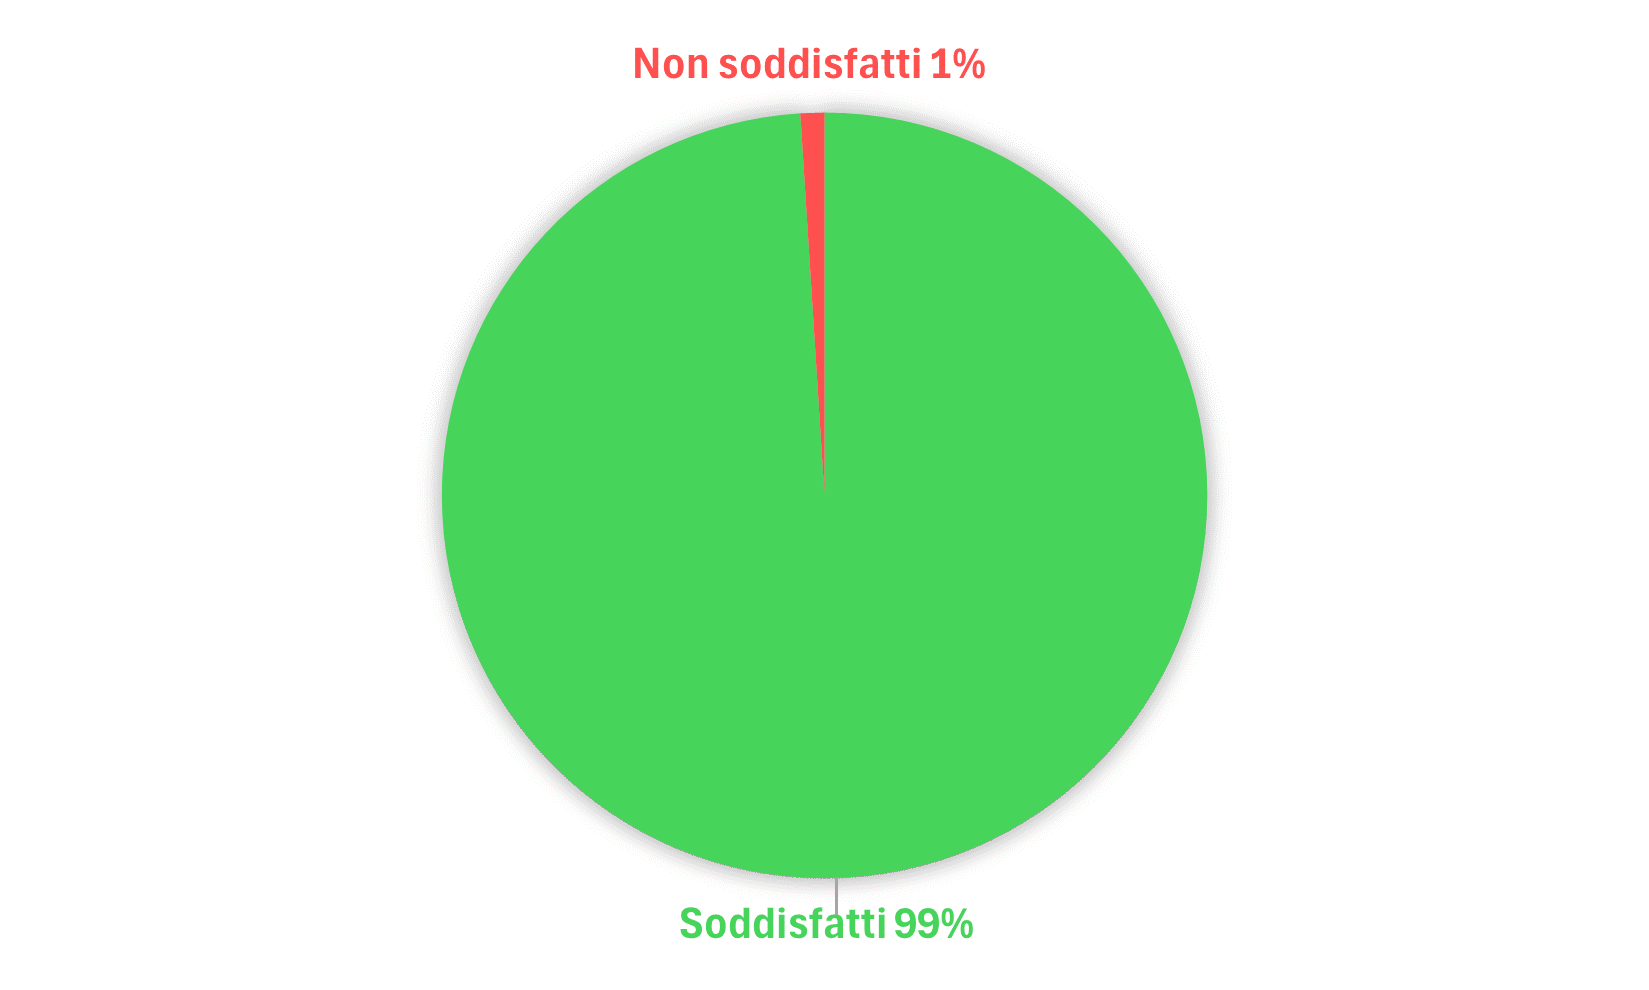
\includegraphics[width=0.8\textwidth]{images_st/torta.png}
    \caption{Grafico dei requisiti soddisfatti.}
    \label{fig:Grafico dei requisiti soddisfatti}
\end{figure}

\end{document}